\section{Funciones}

    Una función, como definición formal, es una regla que asigna a todo
    elemento en el conjunto de partida
    un \textbf{único} elemento en el conjunto de llegada. En si, esta puede verse
    como la relación que hay entre dos conjuntos de números, y se dice que
    una magnitud, numero, es función de otra si el valor de la primera depende
    del valor de la segunda. De esta forma, se obtienen 3 partes fundamentales
    de las funciones:

    \begin{itemize}
        \item Conjunto de partida, dominio:

            Es el conjunto formado por todos los posibles valores que puede \textbf{tomar}
            una función. Corresponde a la \textbf{variable independiente}.

        \item Conjunto de llegada, rango

            Es el conjunto formado por todos los posibles valores que puede \textbf{dar
            como resultado} una función, estos dependen del dominio y la expresión
            que rigen la función. Corresponde a la \textbf{variable dependiente}.

        \item Ecuación la cual rige la función (formula $f(x)= expresión$)

            Esta es una ecuación, la cual puede ser resuelta para una serie de valores
            (dominio) y da como resultado, un conjunto de valores (rango), y cada
            valor en el dominio puede dar un único elemento en el rango.
    \end{itemize}

    Una función suele tener la siguiente forma:

    $$ variable_dependiente = expresión $$

    Donde la expresión viene dada en términos de la variable independiente (una letra), es
    decir, $ expresión= $  \textbf{ecuación en términos de la variable independiente}

    y la variable dependiente puede ser una letra (diferente a la variable independiente)
    o esto: $ f(variable_independiente) $ una $ f $ que representa función, y entre
    corchetes, la variable independientes. Algunos ejemplos son:

    \textbf{Para identificarlas:} La letra que esta sola, a un lado de la
    igualdad es la variable dependiente y la que esta siendo multiplicada, dividida,
    sumada, dentro de una raíz, etc. Es la variable independiente

    $$ f(x) = x^2 $$
    con:

    $ f(x) $: variable dependiente.

    $x$: variable independiente.

    $$ y = x+8 $$
    con:

    $ y $: variable dependiente.

    $x$: variable independiente.

    $$ f(g) = g-95 $$
    con:

    $ f(g) $: variable dependiente.

    $g$: variable independiente.

    $$ h = 975x $$
        con:

    $ h$: variable dependiente.

    $x$: variable independiente.

\subsubsection*{Operaciones con funciones} \label{Operaciones_con_funciones}

    Las funciones pueden ser sumadas, restadas, multiplicadas, divididas
    ,evaluadas y graficadas.


\subsubsection*{Suma y resta de funciones} \label{Suma_de_funciones}

La suma de dos funciones consiste en sumar/restar sus miembros algebraicamente y el
dominio resultante vendrá dado por la intersección de los dominios de las
funciones individuales.

Sean: $ f(x),\ g(x) $ funciones cualesquiera, con sus dominios $ Dom_f,\ Dom_g $

    $$ f(x)\pm g(x)=(f\pm g)(x)= miembros_f + miembros_g $$

y el dominio resultante va a ser dado por:


    $$ Dom_{f\pm g}= Dom_f \cap Dom_g $$


    Ejemplos:

    $ f(x)= 45x,\ Dom_f=\{4,5,8,70,100\} $

    $ g(x)=4 +95x,\ Dom_g= \{1,2,3,5,8,10,100\}$
\\

    $ f(x)+g(x) $

    \begin{align*}
        f(x)+g(x) &= 45x+4+95x 		\\
        f(x)+ g(x)&= 140x + 4
    \end{align*}

    y el dominio viene dado por:
    $$ Dom_{f+g} = Dom_f \cap Dom_g =\{4,5,8,70,100\} \cap \{1,2,3,5,8,10,100\}=\{5,8,100\} $$


    $ f(x)-g(x) $

    \begin{align*}
        f(x)-g(x) &= 45x-(4+95x) 		\\
        f(x)- g(x)&= 45x - 4 -95x\\
        f(x)- g(x)&= -50x - 4
    \end{align*}

    y el dominio viene dado por:
    $$ Dom_{f-g} = Dom_f \cap Dom_g =\{4,5,8,70,100\} \cap \{1,2,3,5,8,10,100\}=\{5,8,100\} $$


    $ g(x)-f(x) $

    \begin{align*}
        g(x)-f(x) &= 45x-(4+95x) 		\\
        g(x)-f(x)&= 45x - 4 -95x\\
        g(x)-f(x)&= -50x - 4
    \end{align*}

    y el dominio viene dado por:
    $$ Dom_{g-f} = Dom_f \cap Dom_g =\{4,5,8,70,100\} \cap \{1,2,3,5,8,10,100\}=\{5,8,100\} $$

\subsubsection*{Multiplicación y división de funciones} \label{Multiplicacion_de_funciones}

La multiplicación/división de funciones se da de la misma forma que la suma o
resta, es decir se multiplican o dividen los términos.

La multiplicación seguirá las propiedades asociativa y/o conmutativa para simplificarse.

En el caso de la división, esta se expresa como una fracción, siendo numerador
y denominador dividendo y divisor respectivamente. Luego se procede a simplificar
si es posible.

Los dominios vienen dados por la intersección en la multiplicación y la intersección
con la exclusión de los puntos donde el denominador se haga 0 en la división
(ya que la división por 0 no esta definida).


Ejemplos:

Sean: $ f(x),\ g(x) $ funciones cualesquiera, con sus dominios $ Dom_f,\ Dom_g $

    $$ f(x) \times g(x)=(f \times g)(x)= miembros_f \times miembros_g $$

y el dominio resultante va a ser dado por:
    $$ Dom_{f\times g}= Dom_f \cap Dom_g $$

    $$ \frac{f(x)}{g(x)}=( \frac{f}{g})(x)= \frac{miembros_f}{miembros_g} $$

y el dominio resultante va a ser dado por:
    $$ Dom_{\frac{f}{g}}= Dom_f \cap Dom_g -\{x|g(x)=0\}$$

    Ejemplos:

    $ f(x)= 45x,\ Dom_f=\{0,-4/95,4,5,8,70,100\} $

    $ g(x)=4 +95x,\ Dom_g= \{0,-4/95, 1,2,3,5,8,10,100\}$


    $ f(x)\times g(x) $

    \begin{align*}
        f(x)\times g(x) &= 45x\times(4+95x)		\\
        f(x)\times g(x) &= 45x\times4 + 45x\times95x\\
        f(x)\times g(x) &= 180x+4275x^2
    \end{align*}

    y el dominio viene dado por:

    $$ Dom_{g\times f} = Dom_f \cap Dom_g =\{0,-4/95,4,5,8,70,100\} \cap \{0,-4/95,1,2,3,5,8,10,100\}=\{0,-4/95,5,8,100\} $$

    $ \frac{f(x)}{g(x)}  $

    \begin{align*}
        \frac{f(x)}{g(x)} &= \frac{45x}{4+95x} 		\\
    \end{align*}

    y el dominio viene dado por:
    $$ Dom_{\frac{f}{g}}= Dom_f \cap Dom_g -\{x|g(x)=0\}$$
    $$ Dom_{\frac{f}{g} } =  (\{0,-4/95,4,5,8,70,100\} \cap \{0,-4/95,1,2,3,5,8,10,100\}) -\{x|4+95x=0  \}$$

    $$Dom_{\frac{f}{g} }=\{0,5,8,100\} $$

$ \frac{g(x)}{f(x)}  $

    \begin{align*}
        \frac{g(x)}{f(x)} &= \frac{4+95x}{45x}		\\
        \frac{g(x)}{f(x)} &= \frac{4}{45x} +\frac{95}{45}
    \end{align*}

    y el dominio viene dado por:
    $$ Dom_{\frac{g}{f}}= Dom_f \cap Dom_g -\{x|f(x)=0\}$$
    $$ Dom_{\frac{g}{f} } =  (\{0,-4/95,4,5,8,70,100\} \cap \{0,-4/95,1,2,3,5,8,10,100\}) -\{x|45x=0 \}$$

    $$Dom_{\frac{f}{g} }=\{-4/95,5,8,100\} $$

\subsubsection*{Evaluación de funciones} \label{Evaluacion_de_funciones}

Es una de las operaciones mas importantes, consiste en sustituir dentro de la
expresión, la variable independiente por un elemento del dominio, esta operación
puede repetirse tantas veces como haga falta con todos los elementos del dominio
para obtener el rango de la función.

Para evaluar una función se escribe de la siguiente forma $ f(a) $, la función
evaluada en le punto $a$, donde $a$ puede ser cualquier elemento o expresión
del dominio de la función.

\textbf{Para realizar esta operación}, se debe sustituir la variable independiente
en la expresión de la función por el termino deseado y luego simplificar de ser
posible.

    Ejemplos:

    Sean:
    $f(x)= 45x$,
    $ g(x)=154 + 75x $  ,
    $ h(x)=\frac{45x}{2} - x^2 $  ,
    $ z(x) = \sqrt[3]{5x+9}  $  .

    Evaluarlas en {0,5,a-2}:

    $f(x)= 45x$

    0: $ f(0)= 45(0)=0$

    5: $ f(5)=45(5)=225 $

    a-2: $ f(a-2)= 45(a-2)=45a-90 $


    $ g(x)=154 + 75x $

    0: $ g(0)=154+75(0)=154 $

    5:  $ g(5)=154+75(5)=154+375=529 $

    a-2: $ g(a-2)=154+75(a-2)=154+75a-150=4+75a $


    $ h(x)=\frac{45x}{2} - x^2 $

    0: $ h(0)=\frac{45(0)}{2} - 0^2 = 0$


    5: $ h(5)=\frac{45(5)}{2} - 5^2 =\frac{225}{2}- 25=\frac{175}{2}  $


    a-2: $ h(a-2)=\frac{45(a-2)}{2} - (a-2)^2= \frac{45a-90}{2} -(a^2-4a+4)=\frac{-2a^2+53a-98}{2}  $


    $ z(x) = \sqrt[3]{5x+9}  $

    0:    $ z(0) = \sqrt[3]{5(0)+9}= \sqrt[3]{9}  $

    5:    $ z(5) = \sqrt[3]{5(5)+9}= \sqrt[3]{34}  $

    a-2:    $ z(a-2) = \sqrt[3]{5(a-2)+9}   = \sqrt[3]{5a-10+9} = \sqrt[3]{5a-1}$

   \subsubsection*{Gráfica de ecuaciones} \label{Grafica_de_ecuaciones}

    La gráfica de una ecuación es el conjunto de puntos (x,y) cuyas coordenadas
    satisfacen la ecuación que define la función. Para esto se evalúan los puntos
    del dominio, tantos sean necesarios para conseguir la forma de la
    ecuación, y posteriormente se unen, mientras mas cercanos sean los puntos entre
    si mas precisa es la gráfica.

    Los puntos se graficar en un \textbf{plano cartesiano}, también conocidas como
    coordenadas rectangulares, esta es una representación bidimensional creada
    por 2 ejes ortogonales ($90^{\circ}$ entre ellos) en donde el eje horizontal
    representa la \textbf{variable independiente} y el eje vertical la \textbf{variable
    dependiente}.

    \begin{tikzpicture}[scale=3,cap=round]
        % Local definitions
        \def\costhirty{0.8660256}
        % Colors
        \colorlet{anglecolor}{green!50!black}
        \colorlet{sincolor}{red}
        \colorlet{tancolor}{orange!80!black}
        \colorlet{coscolor}{blue}
        % Styles
        \tikzstyle{axes}=[]
        \tikzstyle{important line}=[very thick]
        \tikzstyle{information text}=[rounded corners,fill=red!10,inner sep=1ex]
        %The graphic
        \draw[style=help lines,step=0.5cm] (-1.4,-1.4) grid (1.4,1.4);
        \begin{scope}[style=axes]
            \draw[->] (-1.5,0) -- (1.5,0) node[right] {$x$} coordinate(x axis);
            \draw[->] (0,-1.5) -- (0,1.5) node[above] {$y$} coordinate(y axis);
            \foreach \x/\xtext in {-1/-2, -.5/-1,.5/1,1/2}
            \draw[xshift=\x cm] (0pt,1pt) -- (0pt,-1pt) node[below,fill=white] {$\xtext$};
            \foreach \y/\ytext in {-1/-2, -.5/-1,.5/1,1/2}
            \draw[yshift=\y cm] (1pt,0pt) -- (-1pt,0pt) node[left,fill=white] {$\ytext$};
            \draw (.08,-.04) node[ below] {0};
        \end{scope}
    \end{tikzpicture}

    Los puntos que se grafican vienen dados por pares ordenados, estos son objetos
    matemáticos en los que se distingue un elemento y otro donde el primer elemento
    representa el eje x y el segundo el eje y $(x,y)$.

    Ejemplo: Graficar el conjunto de puntos:
    $$ \{ (-3;2), (-2;1), (-1;0), (0;1), (1;1)  \} $$

    Como es un conjunto de puntos, pares ordenados, \textbf{solo deben colocarse
    los puntos, sin unirlos}


    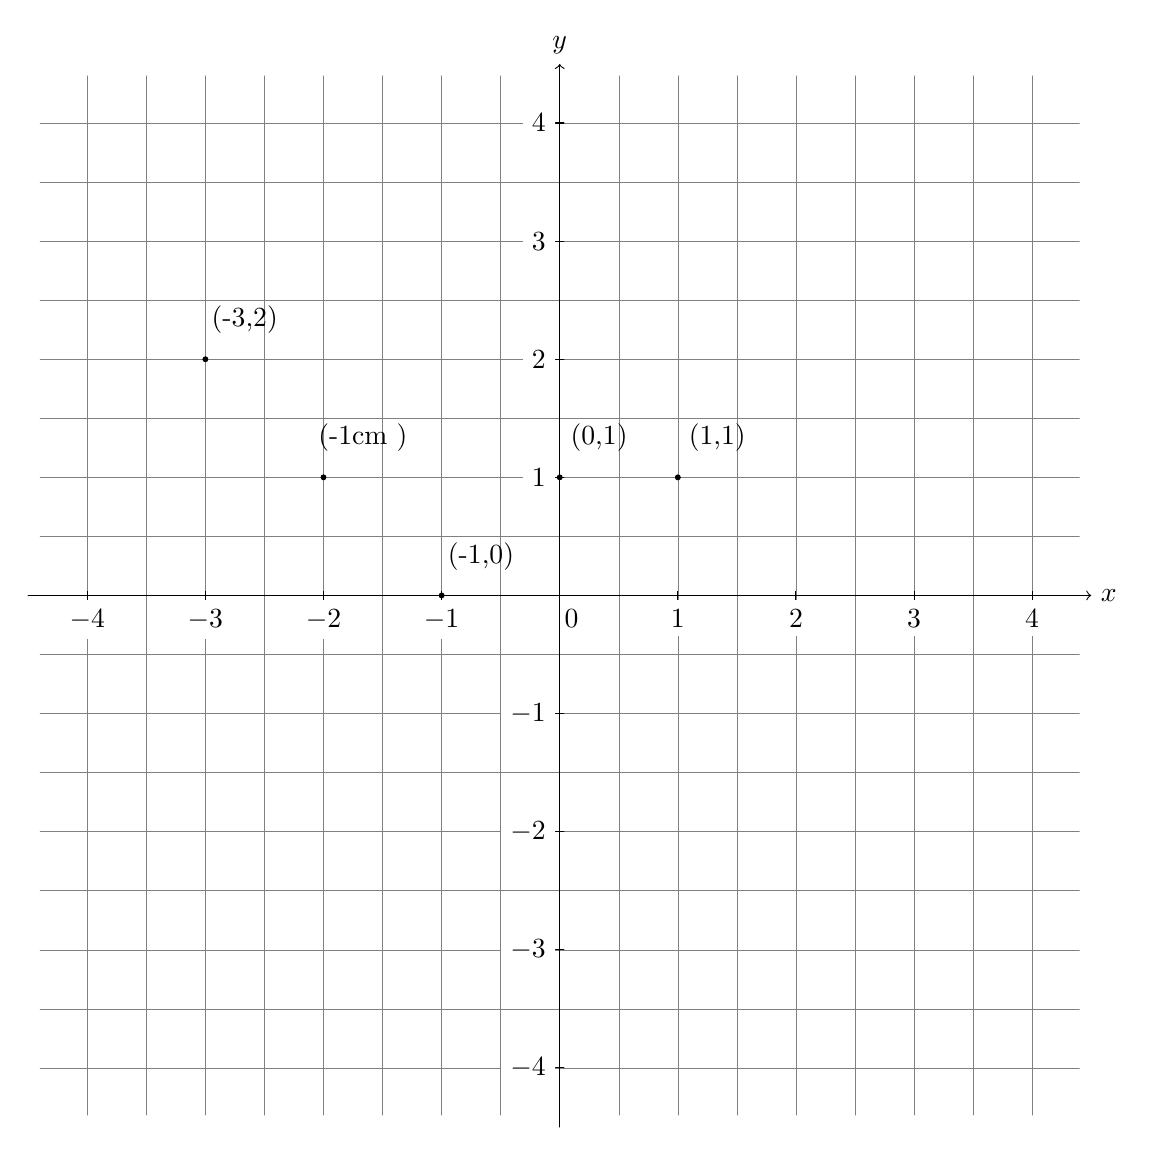
\begin{tikzpicture}[scale=1.5,cap=round]
        % Styles
        \tikzstyle{axes}=[]
        \tikzstyle{important line}=[very thick]
        \tikzstyle{information text}=[rounded corners,fill=red!10,inner sep=1ex]
        %The graphic
        %axes
        \draw[style=help lines,step=0.5cm] (-4.4,-4.4) grid (4.4,4.4);
        \begin{scope}[style=axes]
            \draw[->] (-4.5,0) -- (4.5,0) node[right] {$x$} coordinate(x axis);
            \draw[->] (0,-4.5) -- (0,4.5) node[above] {$y$} coordinate(y axis);
            \foreach \x/\xtext in {-4,-3,-2,-1,1,2,3,4}
            \draw[xshift=\x cm] (0pt,1pt) -- (0pt,-1pt) node[below,fill=white] {$\xtext$};
            \foreach \y/\ytext in {-4,-3,-2,-1,1,2,3,4}
            \draw[yshift=\y cm] (1pt,0pt) -- (-1pt,0pt) node[left,fill=white] {$\ytext$};
            \draw (.1,-.04) node[ below] {0};
        \end{scope}
        %points
        %    \draw (-3,2)-- (-2,1) -- (-1,0) -- (0,1) -- (1,1);
            \filldraw (-3,2) circle (0.02) node[xshift=0.5cm,yshift=0.5cm]{(-3,2)};
            \filldraw (-2,1) circle (0.02) node[xshift=0.5cm,yshift=0.5cm]{(-1cm )};
            \filldraw (-1,0) circle (0.02) node[xshift=0.5cm,yshift=0.5cm]{(-1,0)};
            \filldraw (0,1) circle (0.02) node[xshift=0.5cm,yshift=0.5cm]{(0,1)};
            \filldraw (1,1) circle (0.02) node[xshift=0.5cm,yshift=0.5cm]{(1,1)};
    \end{tikzpicture}

    Si procedemos a unir los puntos, solo se hace cuando es una función,
    obtenemos la siguiente gráfica:

    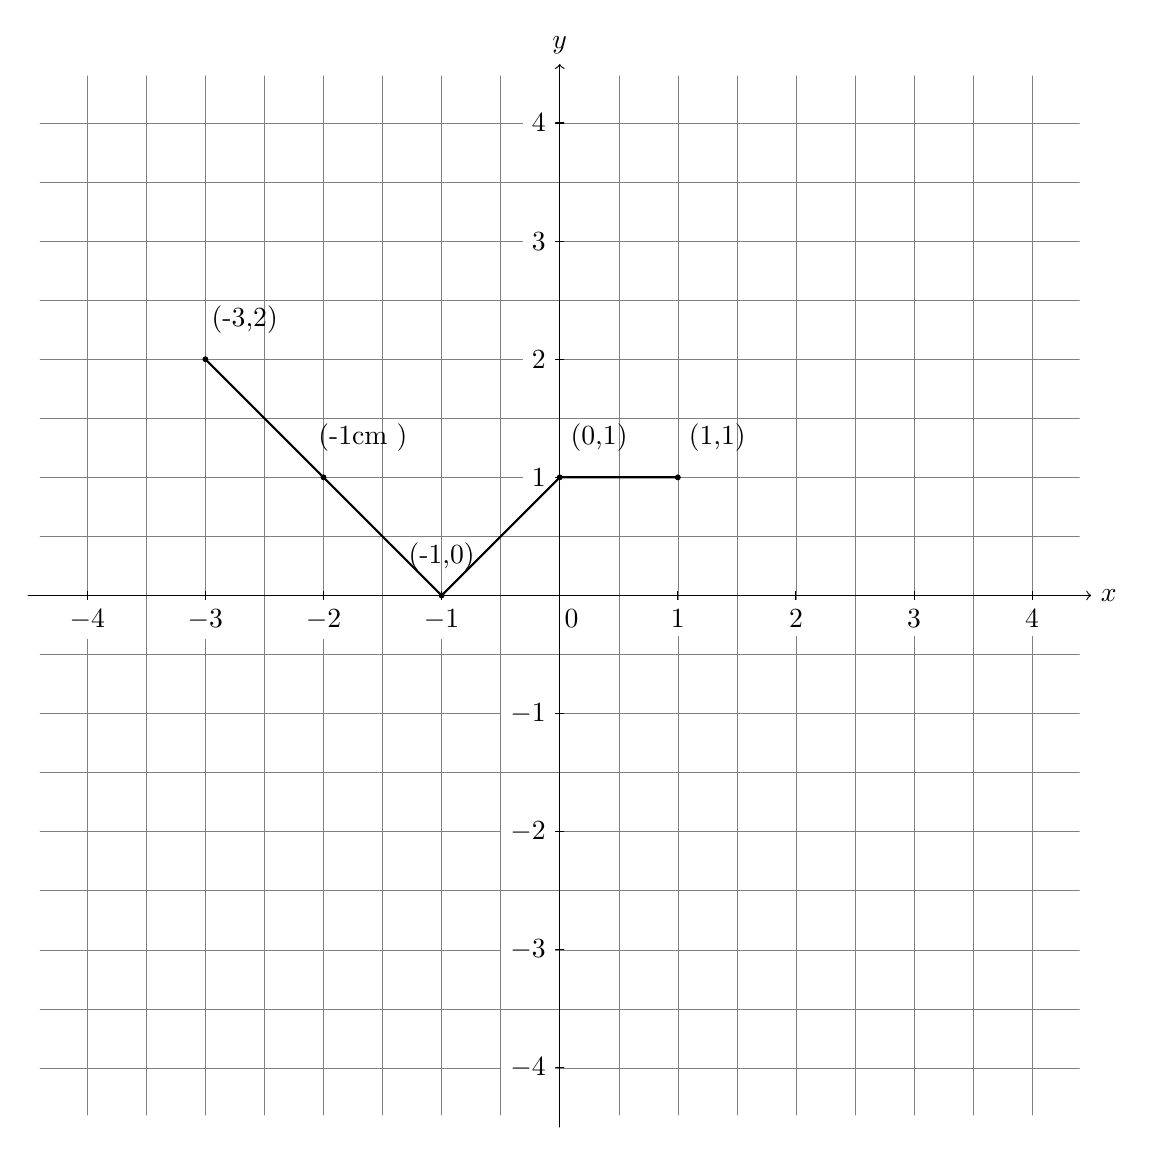
\begin{tikzpicture}[scale=1.5,cap=round]
        % Styles
        \tikzstyle{axes}=[]
        \tikzstyle{important line}=[very thick]
        \tikzstyle{information text}=[rounded corners,fill=red!10,inner sep=1ex]
        %The graphic
        %axes
        \draw[style=help lines,step=0.5cm] (-4.4,-4.4) grid (4.4,4.4);
        \begin{scope}[style=axes]
            \draw[->] (-4.5,0) -- (4.5,0) node[right] {$x$} coordinate(x axis);
            \draw[->] (0,-4.5) -- (0,4.5) node[above] {$y$} coordinate(y axis);
            \foreach \x/\xtext in {-4,-3,-2,-1,1,2,3,4}
            \draw[xshift=\x cm] (0pt,1pt) -- (0pt,-1pt) node[below,fill=white] {$\xtext$};
            \foreach \y/\ytext in {-4,-3,-2,-1,1,2,3,4}
            \draw[yshift=\y cm] (1pt,0pt) -- (-1pt,0pt) node[left,fill=white] {$\ytext$};
            \draw (.1,-.04) node[ below] {0};
        \end{scope}
        %points
            \draw[thick] (-3,2)-- (-2,1) -- (-1,0) -- (0,1) -- (1,1);
            \filldraw (-3,2) circle (0.02) node[xshift=0.5cm,yshift=0.5cm]{(-3,2)};
            \filldraw (-2,1) circle (0.02) node[xshift=0.5cm,yshift=0.5cm]{(-1cm )};
            \filldraw (-1,0) circle (0.02) node[xshift=0cm,yshift=0.5cm]{(-1,0)};
            \filldraw (0,1) circle (0.02) node[xshift=0.5cm,yshift=0.5cm]{(0,1)};
            \filldraw (1,1) circle (0.02) node[xshift=0.5cm,yshift=0.5cm]{(1,1)};
    \end{tikzpicture}

\subsection{Función Lineal}
    Una función lineal es una función polinómica de una variable de primer grado,
    esto implica que es una única variable con exponente 1 y puede estar multiplicada
    por un coeficiente y sumada por una constante (numero).

    Tiene la siguiente forma:

    $$ y = f(x)= mx+b $$
   Donde:

    $ x $  es la variable independiente.

    $ y = f(x) $ es la variable dependiente, puede escribirse de cualquiera
   de las dos formas.

    $m$ es el coeficiente, un numero no nulo ( $ m \not=0 $ ) el cual multiplica
    la variable.

    $ b $ es una constante, es decir un numero que se suma o resta, dependiendo del
    signo, a la variable independiente.

    \textbf{Dominio y Rango}: Ambos son todos los reales, es decir

    $$ Dom_f={\mathbb{R}}\ ;\ Rg_f={\mathbb{R}} $$

    y su gráfica es una linea inclinada con pendiente (inclinación) $ m $  y
    desplazamiento $ b $. Ejemplo:

    $ y=x $

    Procedemos a buscar 2 puntos, es lo mínimo ya que su gráfica es una linea
    recta.

    x=0: y= 0; Par ordenado: (0;0)

    x=1: y=1; Par ordenado: (1;1)

    Graficamos:

    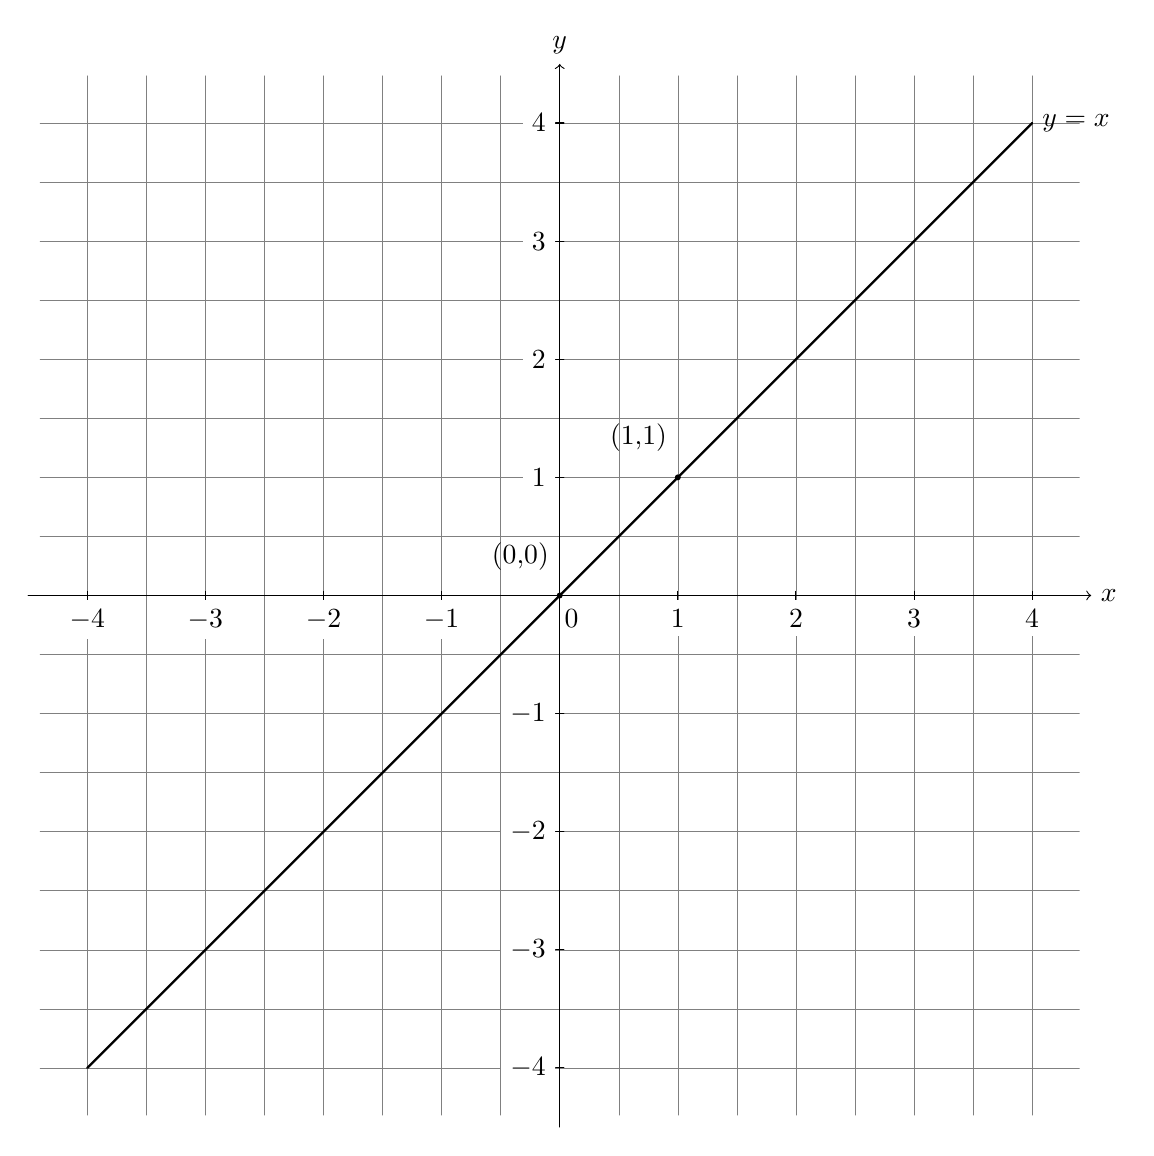
\begin{tikzpicture}[scale=1.5,cap=round]
        % Styles
        \tikzstyle{axes}=[]
        \tikzstyle{important line}=[very thick]
        \tikzstyle{information text}=[rounded corners,fill=red!10,inner sep=1ex]
        %The graphic
        %axes
        \draw[style=help lines,step=0.5cm] (-4.4,-4.4) grid (4.4,4.4);
        \begin{scope}[style=axes]
            \draw[->] (-4.5,0) -- (4.5,0) node[right] {$x$} coordinate(x axis);
            \draw[->] (0,-4.5) -- (0,4.5) node[above] {$y$} coordinate(y axis);
            \foreach \x/\xtext in {-4,-3,-2,-1,1,2,3,4}
            \draw[xshift=\x cm] (0pt,1pt) -- (0pt,-1pt) node[below,fill=white] {$\xtext$};
            \foreach \y/\ytext in {-4,-3,-2,-1,1,2,3,4}
            \draw[yshift=\y cm] (1pt,0pt) -- (-1pt,0pt) node[left,fill=white] {$\ytext$};
            \draw (.1,-.04) node[ below] {0};
        \end{scope}
        %points
            \draw[thick] (-4,-4) -- (4,4)node[right]{$y=x $};
            \filldraw (0,0) circle (0.02) node[xshift=-0.5cm,yshift=0.5cm]{(0,0)};
            \filldraw (1,1) circle (0.02) node[xshift=-0.5cm,yshift=0.5cm]{(1,1)};
    \end{tikzpicture}

    \vspace*{1cm}
    $f(x) = 3x+1$
    Procedemos a buscar 2 puntos

    x=0: y=0+1=1; Par ordenado (0;1)

    x=1: y=3+1; Par ordenado(1;4)


    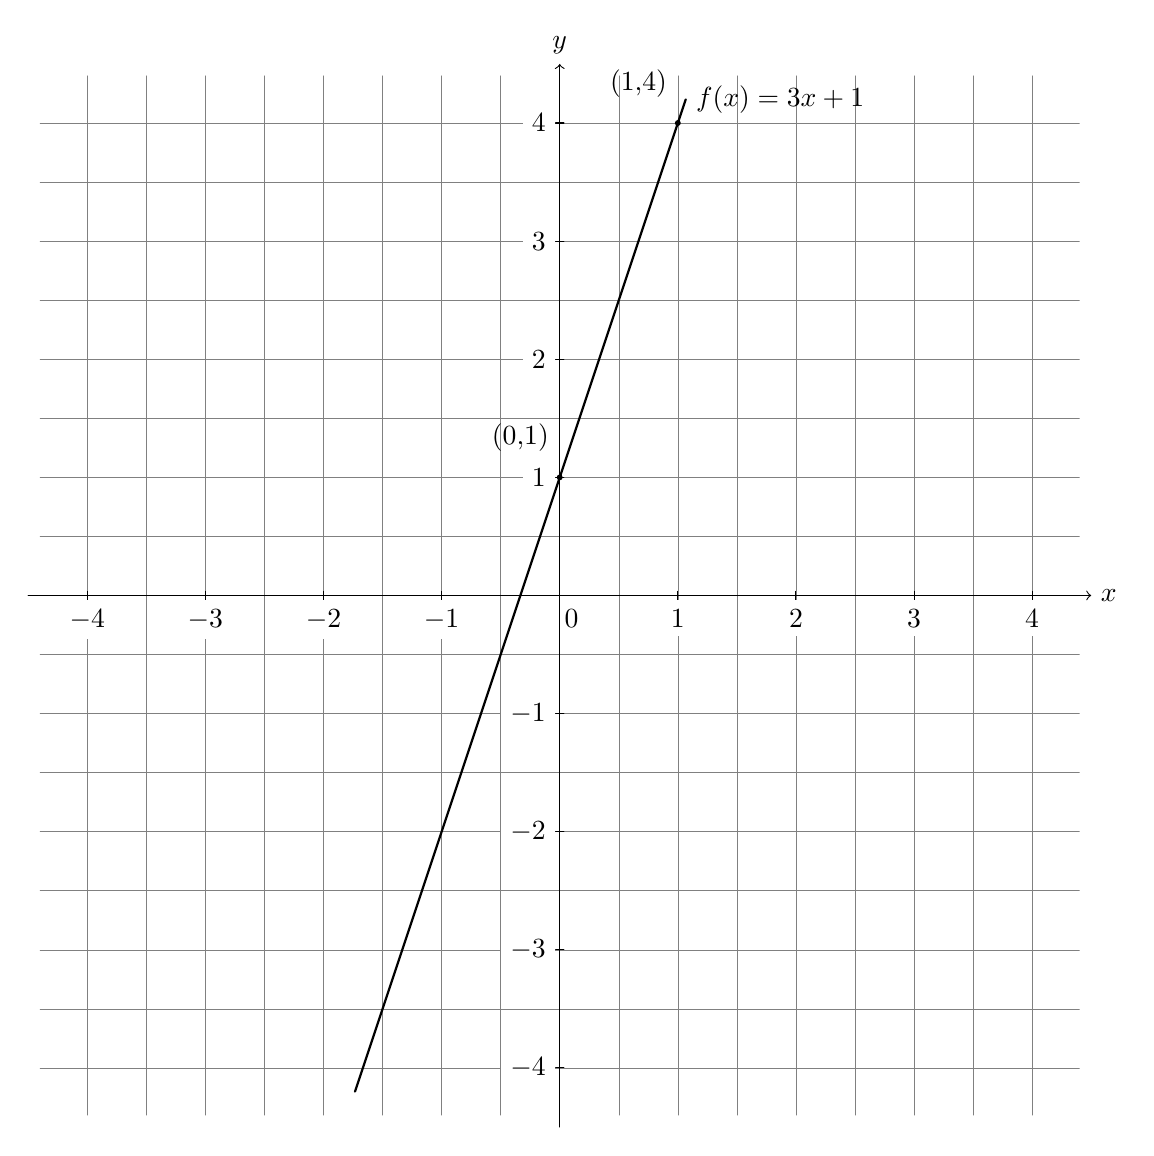
\begin{tikzpicture}[scale=1.5,cap=round]
        % Styles
        \tikzstyle{axes}=[]
        \tikzstyle{important line}=[very thick]
        \tikzstyle{information text}=[rounded corners,fill=red!10,inner sep=1ex]
        %The graphic
        %axes
        \draw[style=help lines,step=0.5cm] (-4.4,-4.4) grid (4.4,4.4);
        \begin{scope}[style=axes]
            \draw[->] (-4.5,0) -- (4.5,0) node[right] {$x$} coordinate(x axis);
            \draw[->] (0,-4.5) -- (0,4.5) node[above] {$y$} coordinate(y axis);
            \foreach \x/\xtext in {-4,-3,-2,-1,1,2,3,4}
            \draw[xshift=\x cm] (0pt,1pt) -- (0pt,-1pt) node[below,fill=white] {$\xtext$};
            \foreach \y/\ytext in {-4,-3,-2,-1,1,2,3,4}
            \draw[yshift=\y cm] (1pt,0pt) -- (-1pt,0pt) node[left,fill=white] {$\ytext$};
            \draw (.1,-.04) node[ below] {0};
        \end{scope}
        %points
            \draw[thick] (-1.7333,-4.2) -- (1.06666,4.2)node[right]{$f(x) = 3x+1 $} ;
            \filldraw (0,1) circle (0.02) node[xshift=-0.5cm,yshift=0.5cm]{(0,1)};
            \filldraw (1,4) circle (0.02) node[xshift=-0.5cm,yshift=0.5cm]{(1,4)};
    \end{tikzpicture}


\subsection{Función Cuadrática}

    una función cuadrática, también conocido como polinomio cuadrático,
    o un polinomio de grado 2,
    es una función polinómica con una variable en la que el término de
    grado más alto es de segundo grado. Esto implica que, después de simplificaciones,
    existen dos variables sumándose, multiplicadas por coeficientes (los cuales no tienen
    que ser iguales) y un termino independiente. Tiene la forma:

    $$ f(x)= ax^2 +bx+c $$

    Donde:
    $ x $  es la variable independiente.
    $a,b,c$ son números reales ($a\not=0$), $ a,b $  son los coeficientes de la
    variable y c es el termino independiente.

    \textbf{Dominio y Rango}: Ambos son todos los reales, es decir

    $$ Dom_f={\mathbb{R}}\ ;\ Rg_f={\mathbb{R}} $$

    \textbf{La gráfica es la misma que la de una parábola}.

    Ejemplos:

    $ f(x)=x^2+x+1 $

    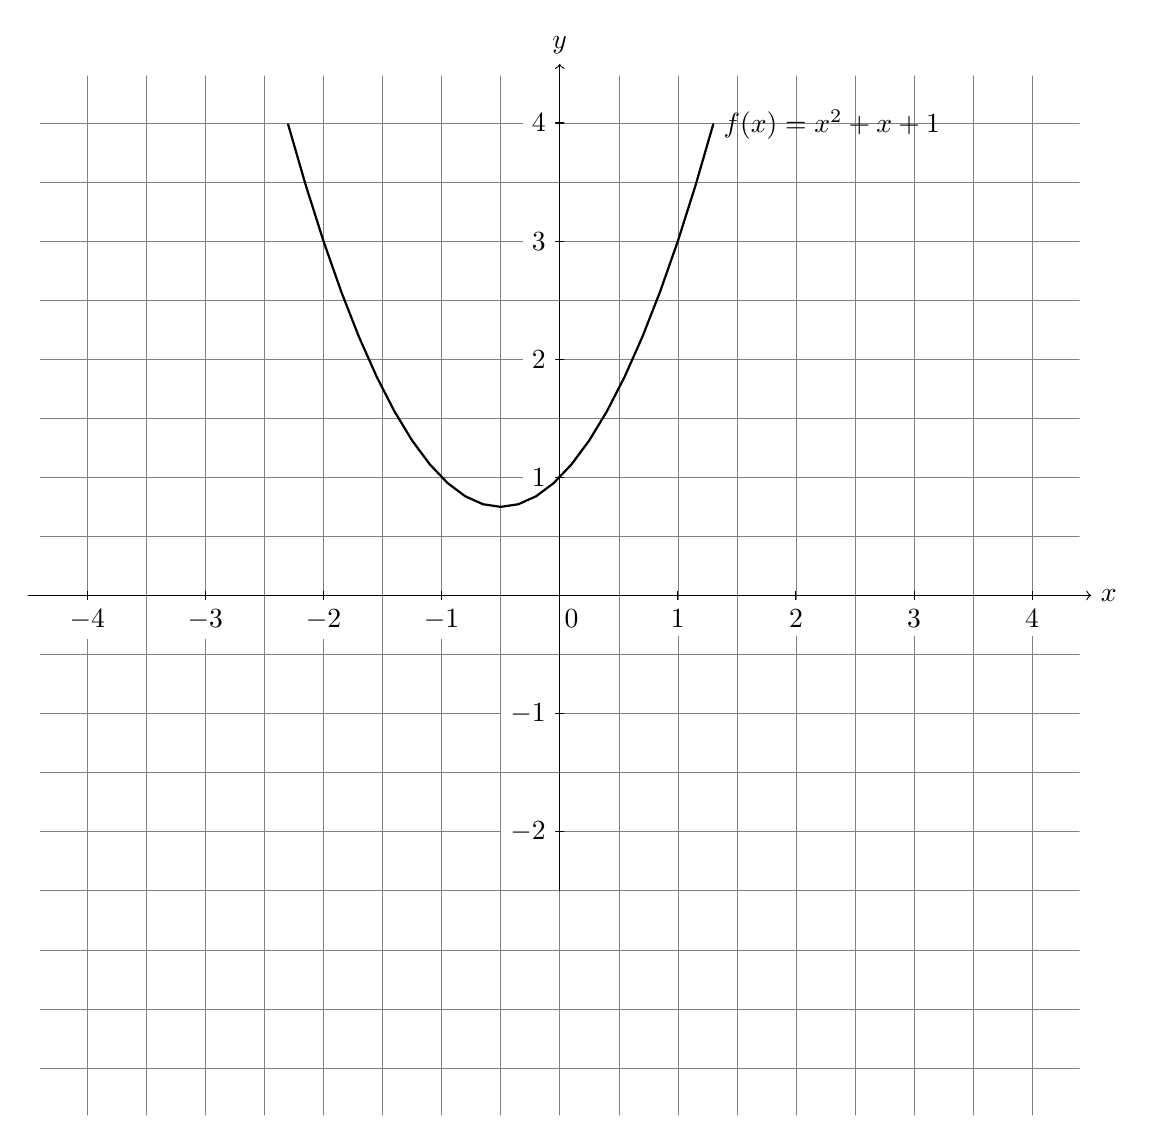
\begin{tikzpicture}[scale=1.5,cap=round]
        % Styles
        \tikzstyle{axes}=[]
        \tikzstyle{important line}=[very thick]
        \tikzstyle{information text}=[rounded corners,fill=red!10,inner sep=1ex]
        %The graphic
        %axes
        \draw[style=help lines,step=0.5cm] (-4.4,-4.4) grid (4.4,4.4);
        \begin{scope}[style=axes]
            \draw[->] (-4.5,0) -- (4.5,0) node[right] {$x$} coordinate(x axis);
            \draw[->] (0,-2.5) -- (0,4.5) node[above] {$y$} coordinate(y axis);
            \foreach \x/\xtext in {-4,-3,-2,-1,1,2,3,4}
            \draw[xshift=\x cm] (0pt,1pt) -- (0pt,-1pt) node[below,fill=white] {$\xtext$};
            \foreach \y/\ytext in {-2,-1,1,2,3,4}
            \draw[yshift=\y cm] (1pt,0pt) -- (-1pt,0pt) node[left,fill=white] {$\ytext$};
            \draw (.1,-.04) node[ below] {0};
        \end{scope}
        %points
            \draw [thick,domain=-2.3:1.3] plot(\x, { (\x)^2 +\x +1  } ) node[right]{$f(x)=x^2+x+1 $} ;
    \end{tikzpicture}

    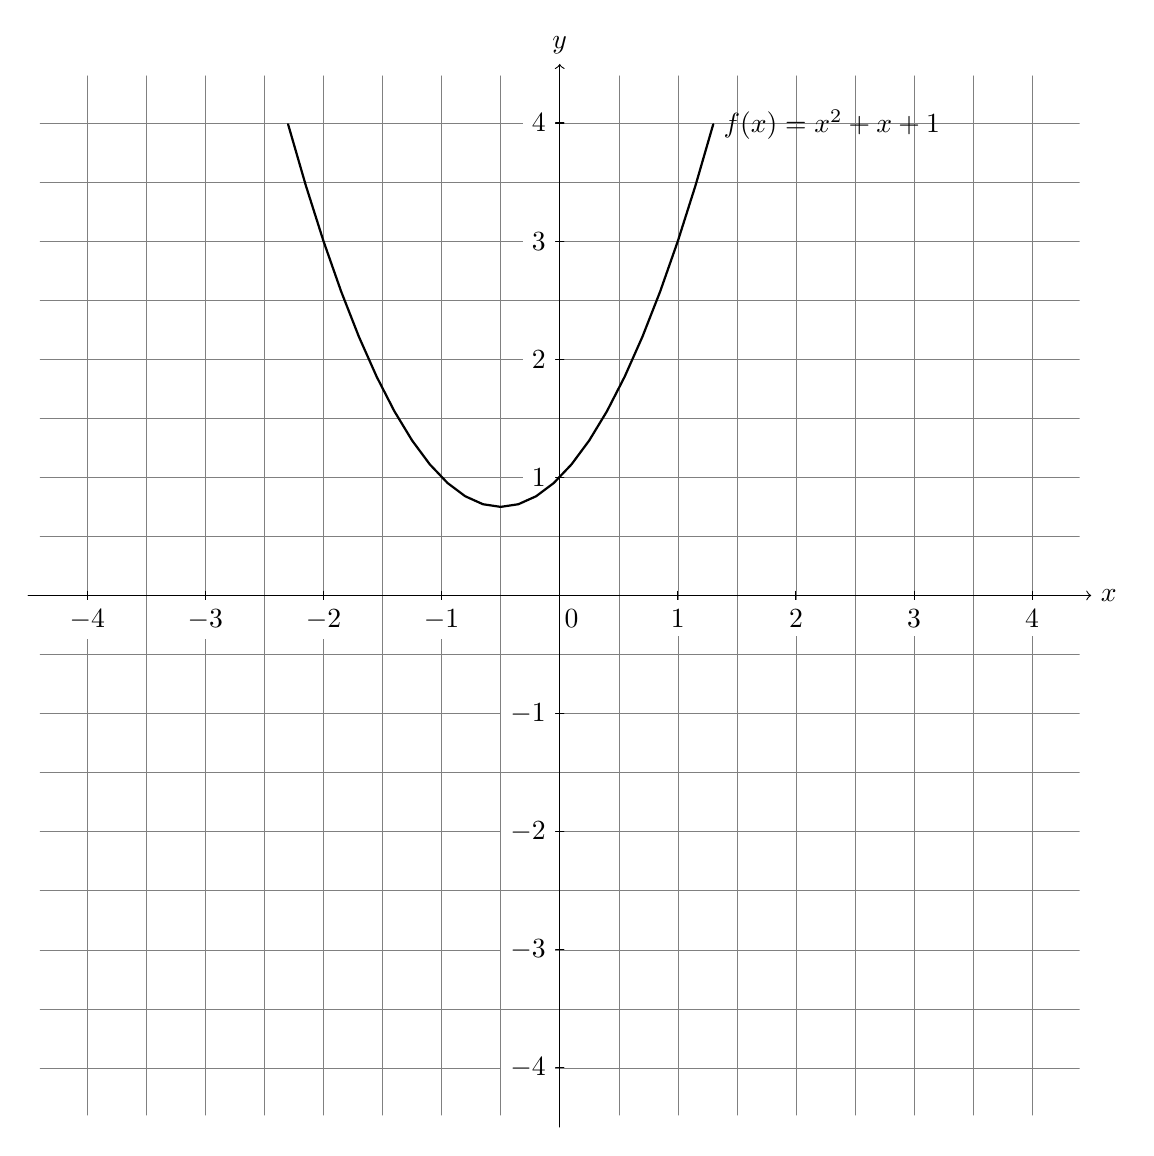
\begin{tikzpicture}[scale=1.5,cap=round]
        % Styles
        \tikzstyle{axes}=[]
        \tikzstyle{important line}=[very thick]
        \tikzstyle{information text}=[rounded corners,fill=red!10,inner sep=1ex]
        %The graphic
        %axes
        \draw[style=help lines,step=0.5cm] (-4.4,-4.4) grid (4.4,4.4);
        \begin{scope}[style=axes]
            \draw[->] (-4.5,0) -- (4.5,0) node[right] {$x$} coordinate(x axis);
            \draw[->] (0,-4.5) -- (0,4.5) node[above] {$y$} coordinate(y axis);
            \foreach \x/\xtext in {-4,-3,-2,-1,1,2,3,4}
            \draw[xshift=\x cm] (0pt,1pt) -- (0pt,-1pt) node[below,fill=white] {$\xtext$};
            \foreach \y/\ytext in {-4,-3,-2,-1,1,2,3,4}
            \draw[yshift=\y cm] (1pt,0pt) -- (-1pt,0pt) node[left,fill=white] {$\ytext$};
            \draw (.1,-.04) node[ below] {0};
        \end{scope}
        %points
            \draw [thick,domain=-2.3:1.3] plot(\x, { (\x)^2 +\x +1  } ) node[right]{$f(x)=x^2+x+1 $} ;
    \end{tikzpicture}

\subsection{Función Polinómica}

    Una función polinómica esta compuesta por una expresión algebraica formada por
    varios monomios (un único termino), En ellos intervienen números y letras
    (ya sea como variable o constantes)
    relacionados mediante sumas, multiplicaciones y potencias.

    Tiene la siguiente forma:

    $$ P(x) = a_nx^n+ a_{n-1}x^n-1+\cdots+ a_1x+a_0 $$

    donde:

    $ P(x) $  es la variable dependiente.

    $x$ es la variable independiente

    $ a_i $con $ i\in {n,n-1,\cdots,1} $  los coeficientes (son los números que
    multiplican a las variables).

    $ a_0 $  el termino independiente.

    Usando una notación mas avanzada, puede escribirse como sumatoria de la forma:


    $$ P(x)= \sum_{i=0}^{n}a_ix^i  $$


    \textbf{El dominio y el rango} son todos los reales es decir:

    $$ Dom_f={\mathbb{R}}\ ;\ Rg_f={\mathbb{R}} $$

    \textbf{La gráfica} es muy variada, no tiene una forma especifica, ya que
    para polinomios de grado 1 tenemos funciones lineales, de grado 2 cuadráticas
    y para grados superiores se hace un estudio exhaustivo para poder graficarlas
    a mano (normalmente se usan graficadoras o programas de computador).

    Algunos ejemplos son:

    $ f(x)= \frac{x^3}{40}+4x^2-x-3 $

    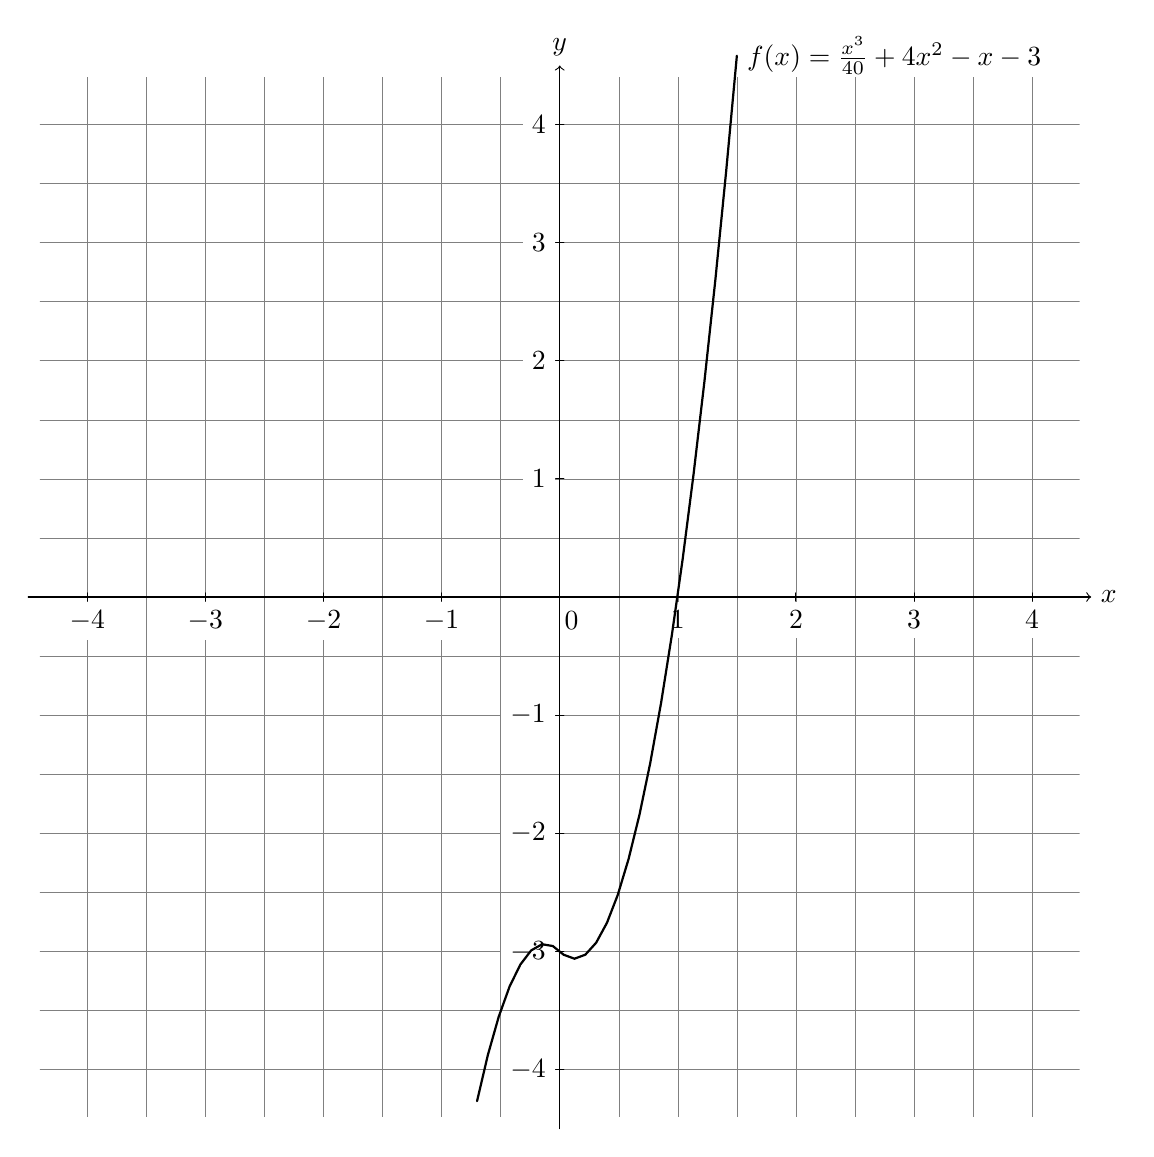
\begin{tikzpicture}[scale=1.5,cap=round]
        % Styles
        \tikzstyle{axes}=[]
        \tikzstyle{important line}=[very thick]
        \tikzstyle{information text}=[rounded corners,fill=red!10,inner sep=1ex]
        %The graphic
        %axes
        \draw[style=help lines,step=0.5cm] (-4.4,-4.4) grid (4.4,4.4);
        \begin{scope}[style=axes]
            \draw[->] (-4.5,0) -- (4.5,0) node[right] {$x$} coordinate(x axis);
            \draw[->] (0,-4.5) -- (0,4.5) node[above] {$y$} coordinate(y axis);
            \foreach \x/\xtext in {-4,-3,-2,-1,1,2,3,4}
            \draw[xshift=\x cm] (0pt,1pt) -- (0pt,-1pt) node[below,fill=white] {$\xtext$};
            \foreach \y/\ytext in {-4,-3,-2,-1,1,2,3,4}
            \draw[yshift=\y cm] (1pt,0pt) -- (-1pt,0pt) node[left,fill=white] {$\ytext$};
            \draw (.1,-.04) node[ below] {0};
        \end{scope}
        %points
            \draw [thick, domain=-0.7:1.5] plot(\x, {0.025*\x^3+4*\x^2-\x-3 } ) node[right]{$f(x)= \frac{x^3}{40}+4x^2-x-3$} ;
    \end{tikzpicture}


$g(x)=-0.1x^5+0.6x^4-0.22x^3-0.54x^2+0.2x+0.48$

    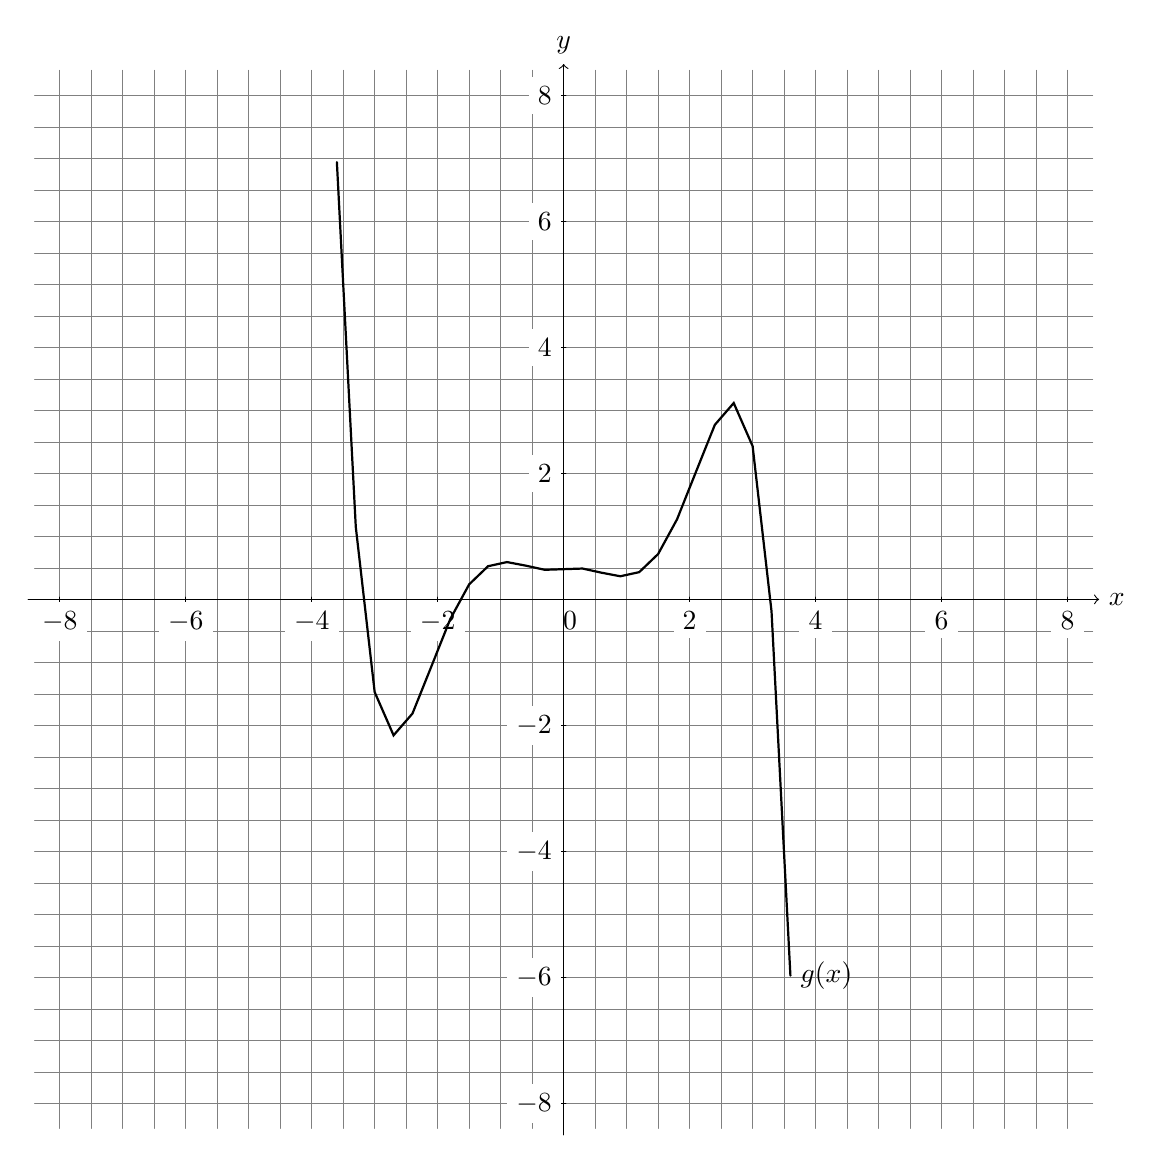
\begin{tikzpicture}[scale=.8,cap=round]
        % Styles
        \tikzstyle{axes}=[]
        \tikzstyle{important line}=[very thick]
        \tikzstyle{information text}=[rounded corners,fill=red!10,inner sep=1ex]
        %The graphic
        %axes
        \draw[style=help lines,step=0.5cm] (-8.4,-8.4) grid (8.4,8.4);
        \begin{scope}[style=axes]
            \draw[->] (-8.5,0) -- (8.5,0) node[right] {$x$} coordinate(x axis);
            \draw[->] (0,-8.5) -- (0,8.5) node[above] {$y$} coordinate(y axis);
            \foreach \x/\xtext in {-8,-6,-4,-2,2,4,6,8}
            \draw[xshift=\x cm] (0pt,1pt) -- (0pt,-1pt) node[below,fill=white] {$\xtext$};
            \foreach \y/\ytext in {-8,-6,-4,-2,2,4,6,8}
            \draw[yshift=\y cm] (1pt,0pt) -- (-1pt,0pt) node[left,fill=white] {$\ytext$};
            \draw (.1,-.04) node[ below] {0};
        \end{scope}
        %points
            \draw [thick, domain=-3.6:3.6] plot(\x, { -0.15*\x^(5)+0.6*\x^(4)-0.22*\x^(3)-0.54*\x^(2)+0.2*\x+0.48} ) node[right]{$g(x)$} ;
    \end{tikzpicture}



\subsection{Cónicas}


    Una \textbf{cónica} o \textbf{sección cónica} es un lugar geométrico que se
    obtiene al intersectar un plano con un cono. Si dicho plano no pasa por el
    vértice, se obtienen las cónicas propiamente dichas. Se clasifican en
    cuatro tipos: elipse, parábola, hipérbola y circunferencia.

    Las curvas cónicas son importantes en la astronomía: dos cuerpos masivos
    que interactúan según la ley universal de la gravitación, describen órbitas
    similares a secciones cónicas: elipses, hipérbolas o parábolas en función
    de sus distancias, velocidades y masas.

    También son muy útiles en aerodinámica y otras aplicaciones industriales,
    ya que permiten ser reproducidas por medios simples con gran exactitud,
    logrando volúmenes, superficies y curvas de gran precisión.

    Cabe resaltar que un cono puede ser visto como un solido en revolución (figura
    3 dimensional que se obtiene al girar una figura plana (2 dimensiones)) obtenido
    a partir de girar un triangulo por sus catetos. También puede ser descrito
    como una función de múltiples variables (3 específicamente), esto atañe a un
    curso de calculo multi variable (Universitario) y por esto solo se nombra.

    \begin{figure}[htb]
 		\centering
		\includegraphics[ width= 8cm ]{Conic_sections_with_plane.png}
        \caption{Secciones generadas por un plano al interactuar un cono.
        \vspace*{0.5cm}
        1. Parábola 2. Elipse y circunferencia 3. hipérbola.}
		\label{secciones}
	\end{figure}


    \subsubsection*{Elipse} \label{Elipse}


    Una elipse es una curva plana, simple y cerrada con dos ejes de
    simetría que resulta al cortar la superficie de un cono por un plano
    oblicuo (inclinado) al eje de simetría con un ángulo mayor que el de la
    generatriz respecto del eje de revolución.

    Es decir es el lugar geométrico de todos los puntos de un plano, tales que
    la suma de las distancias a otros dos puntos fijos, llamados focos, es
    constante.

    Su ecuación, para una elipse horizontal,  es la siguiente:


    $$ \frac{(x-x_o)^2}{a^2} + \frac{(y-y_o)^2}{b^2} = 1 $$

    Donde: $x_0$ y $y_0$ son las coordenadas x e y del centro de la elipse.


    \subsubsection*{Elementos} \label{Elementos}

    Centro: Es el punto de intersección de los ejes. Es, además, centro de
    simetría.

    Eje principal o focal: Es el eje en el que se encuentran los focos. Es un
    eje de simetría.

    Eje secundario: Es el eje perpendicular al eje principal, mediatriz del
    segmento que une los focos.

    Vértices: Puntos de intersección de la elipse con los ejes.

    Distancia focal: Distancia entre los focos. Su longitud es $2\cdot c$.

    Semi-distancia focal: Distancia entre el centro y cada foco. Su longitud es
    $c$.

    Semieje mayor o principal: Segmento entre el centro y los vértices del eje
    principal. Su longitud es $a$.

    Semieje menor o secundario: Segmento entre el centro y los vértices del eje
    secundario. Su longitud es $b$ y cumple $ b= \sqrt{a^2-c^2}  $

    Radio vectores: Cada punto de la elipse cuenta con dos radio vectores que
    son los segmentos que unen dicho punto a cada uno de los focos. Para un
    punto P(x , y) se cumple que $(P , F) = a -e\cdot x y d(P, F') = a+e\cdot x$


    Cabe resaltar que estos conceptos también son aplicables para una elipse
    vertical, si $b>a$ en la ecuación general se produce este cambio, y los focos
    estarían en el eje vertical.


\begin{tikzpicture}
	\draw[very thick] (0,0) ellipse (3cm and 2cm);
	\draw (0,2.25) -- (0,-2.25);
	\draw (3.0,0) -- (-3.25,0);
	\draw[fill, color=blue!30!white] (0,0) -- (0,2) -- (2.236,0) -- cycle;
	\draw[fill] (0,0) circle (0.1);
	\node at (0.25,0.25) {\small C};
    \draw[fill] (0,2.0) circle (0.1);
    \node[color=blue] at (0.25,2.25) {\small b};
    \draw[fill] (0,-2.0) circle (0.1);
    \node[color=blue] at (-0.25,-2.25) {\small -b};
    \node[color=blue] at (3.25,0.15) {\small a};
    \node[color=blue] at (-3.25,0.15) {\small -a};
    \node[color=red!75!black] at (-2.35,0.25) {\small F1};
    \node[color=red!75!black] at (2.35,0.25) {\small F2};
    \node[color=red!75!black] at (1.175,-0.25) {\small c};
    \node[color=red!75!black] at (1.1,1.25) {\small a};
    \node[color=red!75!black] at (-0.25,0.9) {\small b};
    \node[color=green!75!black] at (1.1,2.15) {\small P};
    \draw[color=green!75!black] (1.0,1.885618) -- (-2.236,0);
    \draw[color=green!75!black] (1.0,1.885618) -- (2.236,0);
    \draw[color=blue!75!black,dashed, very thick] (4.0249,2.5) -- (4.0249,-2.5);
    \node[color=blue!75!black] at (4.75,1.0) {$x=\dfrac{a^2}{c}$};
    \draw[color=blue!75!black,very thick] (1.0,1.885618) -- (4.0,1.885618);
    \draw[fill, blue!75!black] (4.0,1.885618) circle (0.1);
    \node[color=blue!75!black] at (4.25,1.88) {\small D};
    \draw[color=blue!75!black] (3.0,0) -- (4.0,0);
    \draw[fill, blue!75!black] (4.0,0) circle (0.1);
    \node[color=blue!75!black] at (4.25,0) {\small d};
    \draw[fill] (3.0,0) circle (0.1); %punto a
    \draw[fill] (-3.0,0) circle (0.1); %punto -a
    \draw[fill, red!75!black] (-2.236,0) circle (0.1); %punto F1
    \draw[fill, red!75!black] (2.236,0) circle (0.1); %punto F2
    \draw[fill, green!75!black] (1.0,1.885618) circle (0.1); %punto P
\end{tikzpicture}




    \subsubsection*{Parábola} \label{Parábola}

    una parábola  es la sección cónica de excentricidad
    igual a 1,resultante de cortar un cono recto con un plano cuyo
    ángulo de inclinación respecto al eje de revolución del cono sea igual al
    presentado por su generatriz.

    Se denomina parábola al lugar geométrico de un punto que se mueve en un
    plano de tal manera que equidista de una recta fija, llamada directriz y de
    un punto fijo en el plano, que no pertenece a la parábola ni a la
    directriz, llamado foco.

    Su gráfica es muy parecida a la del polinomio de orden 2 y su ecuación tiene
    la forma:

    $$ (y-y_o)^2 =2p(x-x_o) $$

    Donde: $x_0$ y $y_0$ son las coordenadas x e y del centro de la parábola.

    \subsubsection*{Elementos} \label{Elementos}

    Eje: Es un eje de simetría y por donde pasa el foco

    foco: Punto equidistante a todo par de puntos (simétricos)  de la parábola

    Vértice: Puntos de intersección de la parábola con el eje.

    directriz: Recta equidistante a los puntos de la parábola.


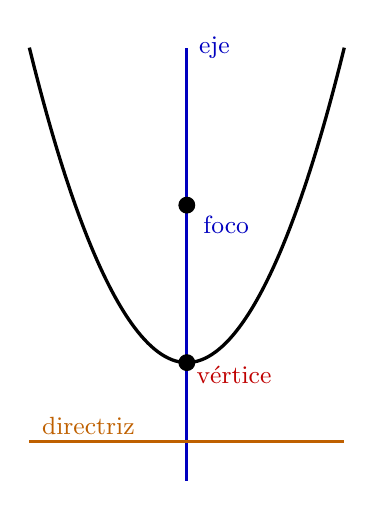
\begin{tikzpicture}
	\draw[very thick](0,-2) parabola (-2,2) (0,-2) parabola (2,2);
	\node[color=red!75!black] at (0.6,-2.15) {\small vértice};
	\draw[very thick,blue!75!black](0,-3.5) -- (0,2);
	\node[color=blue!75!black] at (0.35,2.0) {\small eje};
	\node[color=blue!75!black] at (0.5,-0.25) {\small foco};
	\draw[very thick,orange!75!black](-2,-3) -- (2,-3);
	\node[color=orange!75!black] at (-1.25,-2.8) {\small directriz};
	\draw[fill] (0,-2) circle (0.1);
	\draw[fill] (0,0) circle (0.1);
\end{tikzpicture}



    \subsubsection*{hipérbola} \label{hipérbola}

    Una hipérbola  es una curva abierta de dos ramas,
    obtenida cortando un cono recto mediante un plano no necesariamente
    paralelo al eje de simetría, y con ángulo menor que el de la generatriz
    respecto del eje de revolución.

    También se define como se define como el lugar geométrico de los puntos del
    plano en el que la diferencia de distancias a dos puntos fijos denominados
    focos, F y F', es siempre constante.

    Una hipérbola horizontal es descrita por la ecuación:

    $$ \frac{(x-x_o)^2}{a^2} - \frac{(y-y_o)^2}{b^2} = 1 $$

    Donde: $x_0$ y $y_0$ son las coordenadas x e y del centro de la hipérbola.

   \subsubsection*{Elementos} \label{Elementos}

    Centro: Es el punto de $o$, el centro de simetría.

    Eje principal o focal: Es el eje en el que se encuentran los focos. Es un
    eje de simetría.

    Eje secundario: Es el eje perpendicular al eje principal, mediatriz del
    segmento que une los focos.

    Vértices: Puntos de intersección de las hipérbolas con el eje focal.

    Distancia focal: Distancia entre los focos.

    Semi-distancia focal: Distancia entre el centro y cada foco.


    \begin{figure}[htb]
 		\centering
		\includegraphics[ width= 8cm ]{Hiperbola.png}
        \vspace*{0.5cm}
	\end{figure}


    \subsubsection*{Circunferencia} \label{Circunferencia}

    La circunferencia es una curva plana y cerrada tal que todos sus puntos
    están a igual distancia del centro.

    Una circunferencia es el lugar geométrico de los puntos de un plano que
    equidistan a otro punto llamado centro.

    La circunferencia es descrita por la ecuación:


    $$ (x-x_0)^2+(y-y_0)^2 = r^2 $$


    Donde: $x_0$ y $y_0$ son las coordenadas x e y del centro de la circunferencia.
    $r$ es el radio de la circunferencia.

    \subsubsection*{Elementos} \label{Elementos}

    El centro es el punto equidistante a todos los puntos de una
    circunferencia. Señalado con el nombre  C en la figura.

    Radio es cualquier segmento que une el centro de la circunferencia con
    un punto cualquiera de la misma. El radio también es la longitud de los
    segmentos del mismo nombre.

    Un  diámetro es cualquier segmento que une dos puntos de la circunferencia
    pasando por su centro. El diámetro también es la longitud de los segmento
    del mismo nombre.

    El perímetro es el contorno de la circunferencia y su longitud.

    Una cuerda es cualquier segmento que une dos puntos de una circunferencia.
    El diámetro es una cuerda de máxima longitud.

    Un arco es cualquier porción de circunferencia delimitada por dos puntos
    sobre esta. Se dice también que una cuerda subtiende cada arco que
    determinan sus extremos.


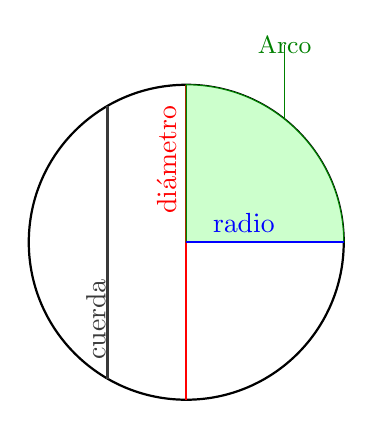
\begin{tikzpicture}
	\draw[thick] (0,0) circle (2cm);
	\draw[red, thick] (0,-2) -- (0,2) node[right=-0.5cm, below=0.95cm, semithick, rotate=90] {diámetro}; %diámetro
	\filldraw[fill=green!20!white,draw=green!50!black](0,0)--(2cm,0) arc (0:90:2cm)--cycle; %arco
	\draw [green!50!black](1.25,1.55) -- (1.25,2.5) node {\small  Arco};
	\draw[blue, thick] (0,0) -- (2,0) node[above=0.25cm, left=0.75cm, semithick] {radio}; %radio
	\draw[gray!45!black, thick] (-1,1.732) -- (-1,-1.732) node[right=0.1cm, above=0.75cm, semithick, rotate=90] {cuerda}; %cuerda
\end{tikzpicture}



\subsection{Función Exponencial}

    una función exponencial es una función de la forma
    $$f(x)=ab^{x}$$
    en el que el argumento $x$ se presenta como un exponente.

    $b$ es la base.

    $a$ es el coeficiente que multiplica a la base.

    Cabe destacar que una función de la forma  $f(x)=ab^{cx+d}$ también es una función
    exponencial, ya que puede reescribirse como: $ ab^{cx+d} = (a b^d)(b^c)^x $

    \textbf{Dominio}: Todos los reales. $ \mathbb{R} $

    \textbf{Rango}: Todos los reales positivos sin incluir el 0 {$\mathbb{R}^+ -\{0\} $}

    Ejemplos:

    Para la función $ f(x)= 2^x $


    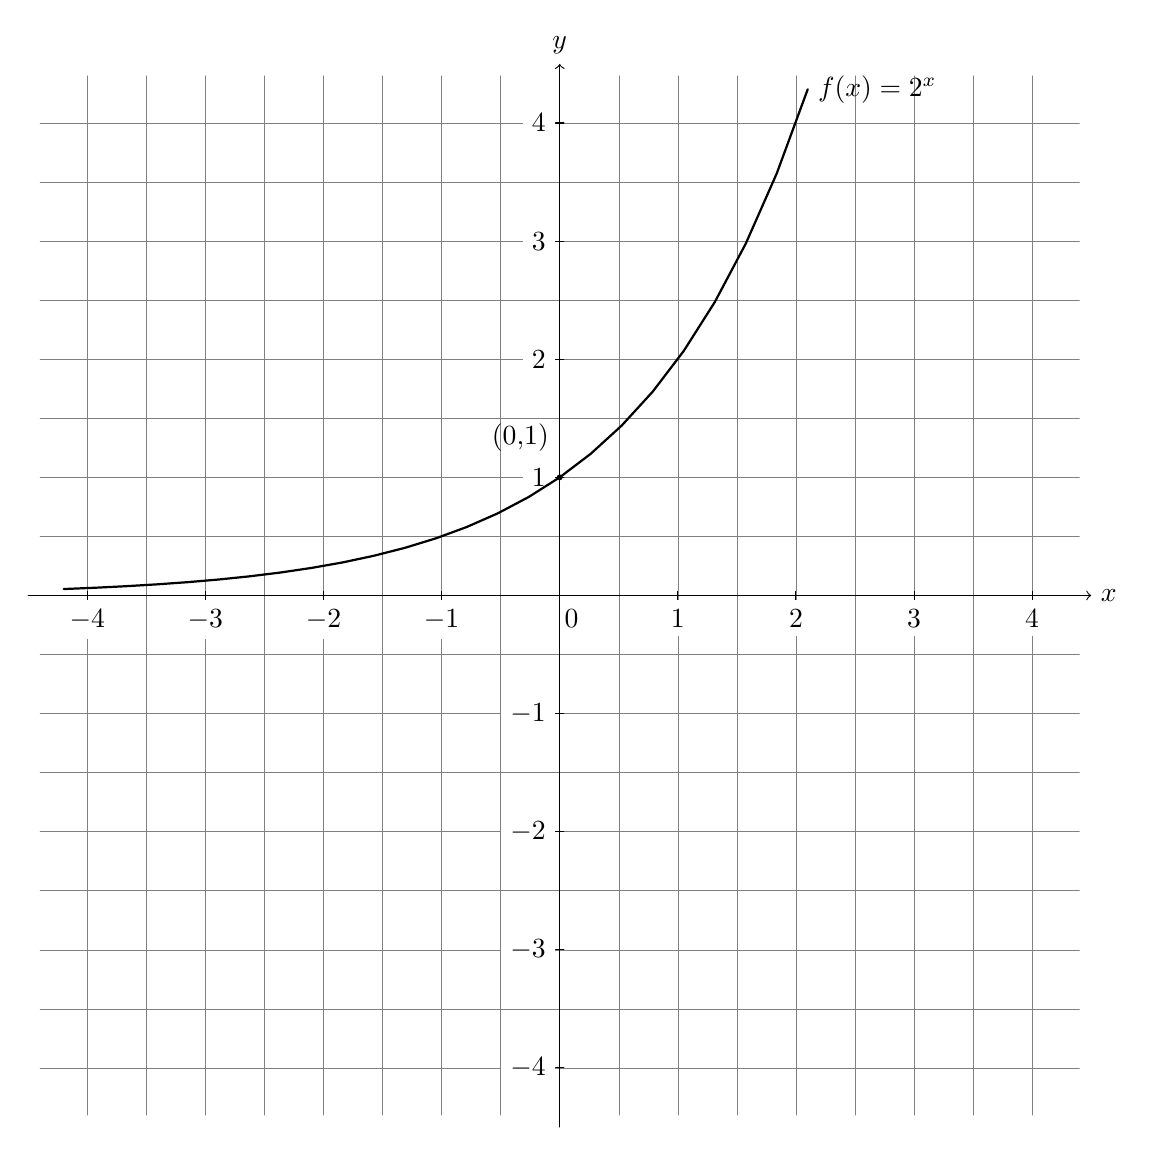
\begin{tikzpicture}[scale=1.5,cap=round]
        % Styles
        \tikzstyle{axes}=[]
        \tikzstyle{important line}=[very thick]
        \tikzstyle{information text}=[rounded corners,fill=red!10,inner sep=1ex]
        %The graphic
        %axes
        \draw[style=help lines,step=0.5cm] (-4.4,-4.4) grid (4.4,4.4);
        \begin{scope}[style=axes]
            \draw[->] (-4.5,0) -- (4.5,0) node[right] {$x$} coordinate(x axis);
            \draw[->] (0,-4.5) -- (0,4.5) node[above] {$y$} coordinate(y axis);
            \foreach \x/\xtext in {-4,-3,-2,-1,1,2,3,4}
            \draw[xshift=\x cm] (0pt,1pt) -- (0pt,-1pt) node[below,fill=white] {$\xtext$};
            \foreach \y/\ytext in {-4,-3,-2,-1,1,2,3,4}
            \draw[yshift=\y cm] (1pt,0pt) -- (-1pt,0pt) node[left,fill=white] {$\ytext$};
            \draw (.1,-.04) node[ below] {0};
        \end{scope}
        %points
            \draw [thick,domain=-4.2:2.1] plot(\x, { 2^\x  } ) node[right]{$f(x)= 2^x  $} ;
            \filldraw (0,1) circle (0.02) node[xshift=-0.5cm,yshift=0.5cm]{(0,1)};
    \end{tikzpicture}

    Otros ejemplos:

    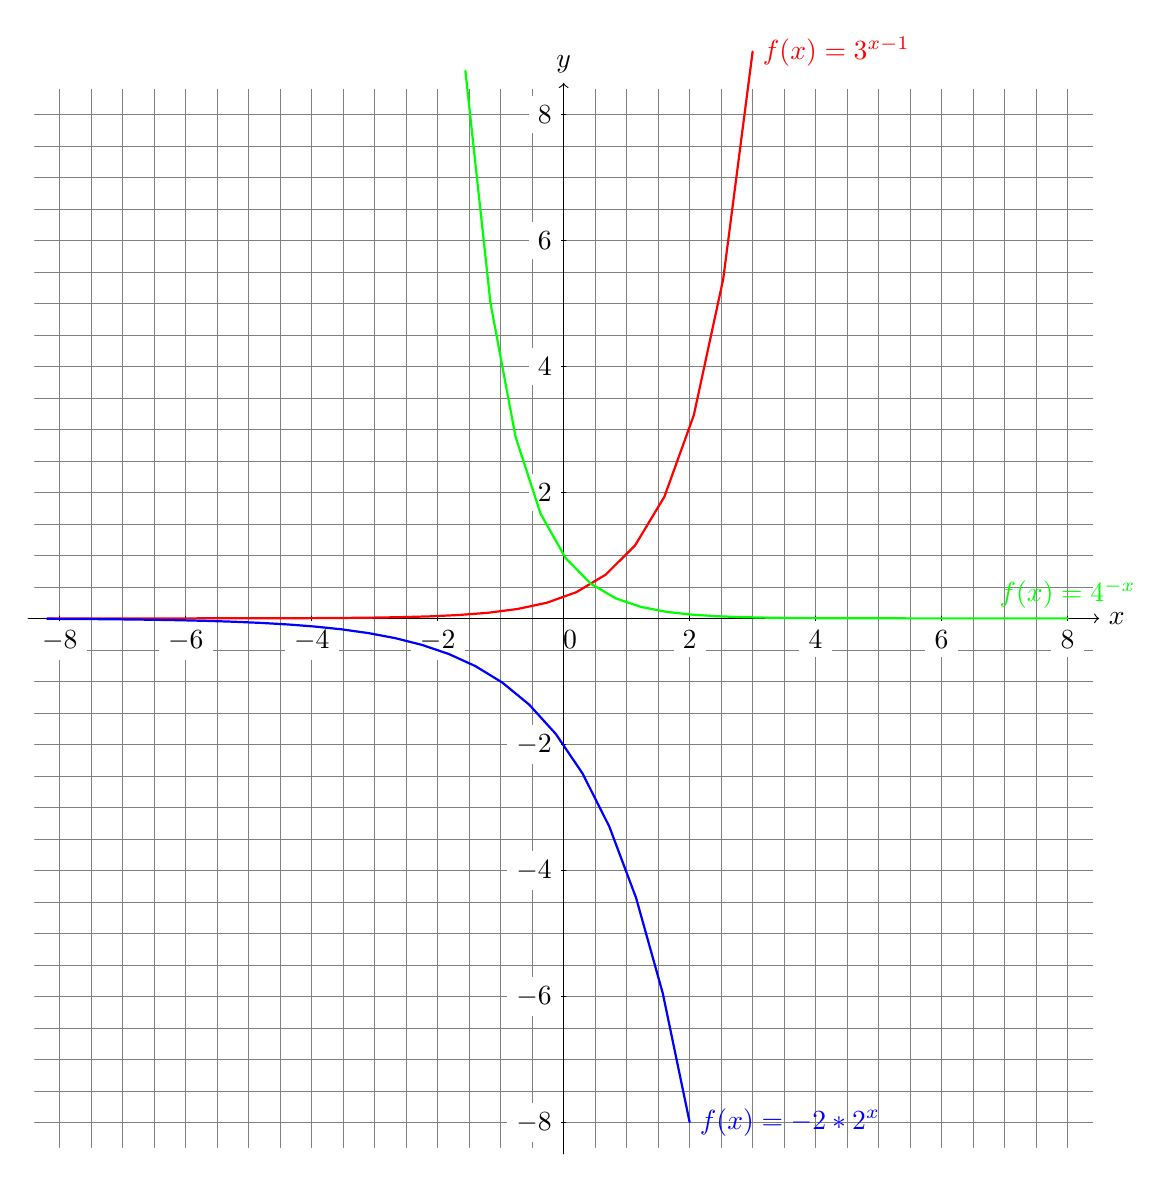
\begin{tikzpicture}[scale=.8,cap=round]
        % Styles
        \tikzstyle{axes}=[]
        \tikzstyle{important line}=[very thick]
        \tikzstyle{information text}=[rounded corners,fill=red!10,inner sep=1ex]
        %The graphic
        %axes
        \draw[style=help lines,step=0.5cm] (-8.4,-8.4) grid (8.4,8.4);
        \begin{scope}[style=axes]
            \draw[->] (-8.5,0) -- (8.5,0) node[right] {$x$} coordinate(x axis);
            \draw[->] (0,-8.5) -- (0,8.5) node[above] {$y$} coordinate(y axis);
            \foreach \x/\xtext in {-8,-6,-4,-2,2,4,6,8}
            \draw[xshift=\x cm] (0pt,1pt) -- (0pt,-1pt) node[below,fill=white] {$\xtext$};
            \foreach \y/\ytext in {-8,-6,-4,-2,2,4,6,8}
            \draw[yshift=\y cm] (1pt,0pt) -- (-1pt,0pt) node[left,fill=white] {$\ytext$};
            \draw (.1,-.04) node[ below] {0};
        \end{scope}
        %points
            \draw [thick,color= red, domain=-8.2:3] plot(\x, { 3^(\x-1)  } ) node[right]{$f(x)= 3^{x-1}  $} ;
            \draw [thick,color = blue, domain=-8.2:2] plot(\x, { -2*(2)^(\x)  } ) node[right]{$f(x)=-2*2^{x}  $} ;
            \draw [thick,color= green, domain=-1.56:8] plot(\x, { 4^(-1*\x)  } ) node[above]{$f(x)= 4^{-x}  $} ;
    \end{tikzpicture}


\subsection{Función Logarítmica}

    Una función logarítmica es una función la cual esta formada por un logaritmo
    de base a y tiene la forma:


    $$ f(x)= \log_{a}{x} $$

    donde:
    $x$ es la variable independiente.
    $\log_{a}$ es un logaritmo, la inversa de la función exponencial y tiene como
    base el numero $a$, este puede ser un numero real positivo, distinto de 0 y 1
    es decir: $ a \in \{ \mathbb{R}: 0<a \^ a \not = 1   \} $

    \textbf{Cabe destacar que}: x puede ser otra función, un argumento, sumas,
    multiplicaciones, etc.

    $$ f(x)= \log_{a}{arg(x)} $$

    \textbf{El dominio} son todos los números reales que hacen que el argumento
    anteriormente nombrado sea mayor que 0, entonces $ Dom_f=\{x:arg(x)\in\ \mathbb{R}^{+}-\{0\}\} $

    \textbf{El rango}: son todos los números reales.

    La gráfica, para $\log_e(x)$ el cual es conocido como logaritmo natural
    o neperiano, viene dada por:

    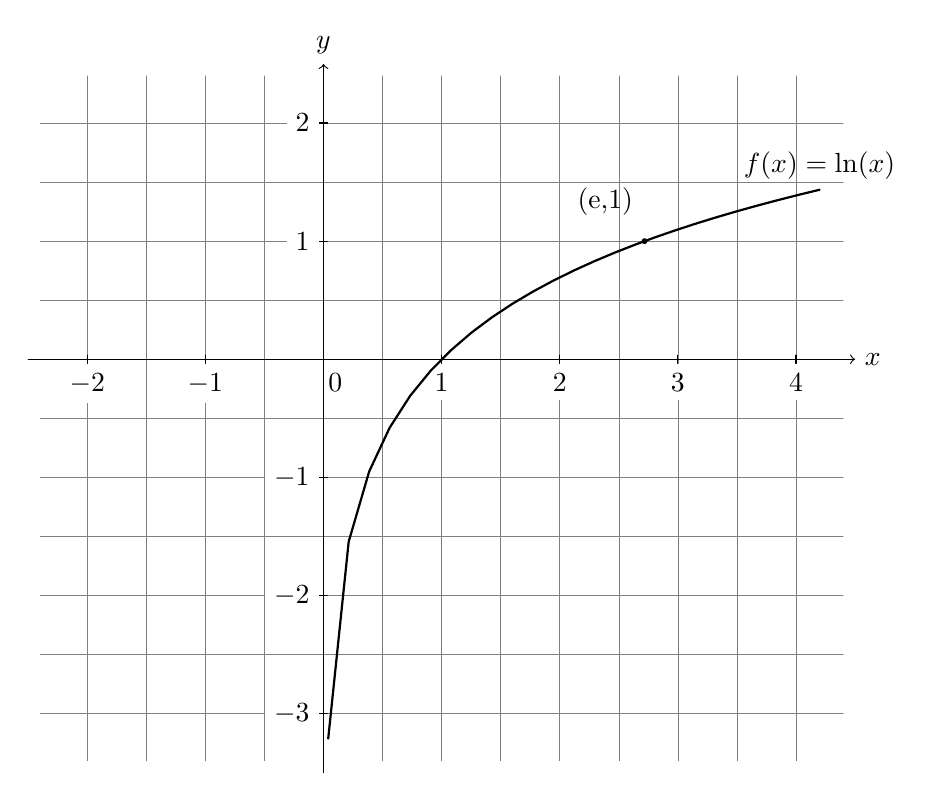
\begin{tikzpicture}[scale=1.5,cap=round]
        % Styles
        \tikzstyle{axes}=[]
        \tikzstyle{important line}=[very thick]
        \tikzstyle{information text}=[rounded corners,fill=red!10,inner sep=1ex]
        %The graphic
        %axes
        \draw[style=help lines,step=0.5cm] (-2.4,-3.4) grid (4.4,2.4);
        \begin{scope}[style=axes]
            \draw[->] (-2.5,0) -- (4.5,0) node[right] {$x$} coordinate(x axis);
            \draw[->] (0,-3.5) -- (0,2.5) node[above] {$y$} coordinate(y axis);
            \foreach \x/\xtext in {-2,-1,1,2,3,4}
            \draw[xshift=\x cm] (0pt,1pt) -- (0pt,-1pt) node[below,fill=white] {$\xtext$};
            \foreach \y/\ytext in {-3,-2,-1,1,2}
            \draw[yshift=\y cm] (1pt,0pt) -- (-1pt,0pt) node[left,fill=white] {$\ytext$};
            \draw (.1,-.04) node[ below] {0};
        \end{scope}
        %points
            \draw [thick,domain=0.04:4.2] plot(\x, { ln(\x ) } )node[above]{$f(x)= \ln(x) $};
            \filldraw (2.7182,1) circle (0.02) node[xshift=-0.5cm,yshift=0.5cm]{(e,1)};
    \end{tikzpicture}


    Otros ejemplos:


    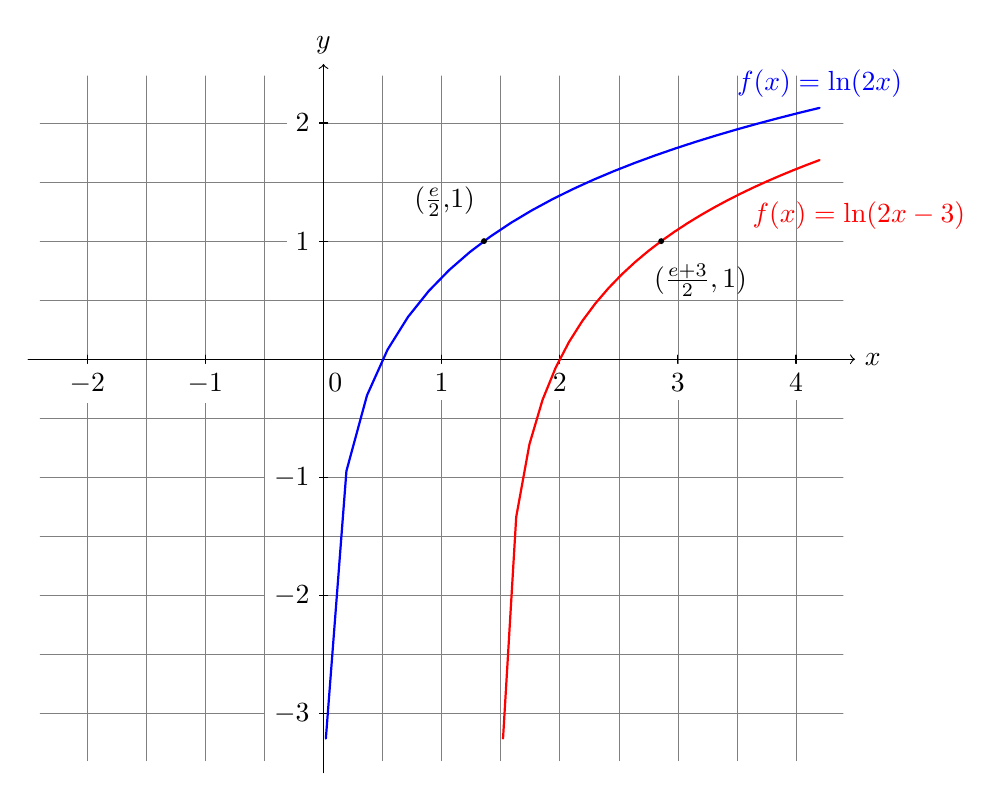
\begin{tikzpicture}[scale=1.5,cap=round]
        % Styles
        \tikzstyle{axes}=[]
        \tikzstyle{important line}=[very thick]
        \tikzstyle{information text}=[rounded corners,fill=red!10,inner sep=1ex]
        %The graphic
        %axes
        \draw[style=help lines,step=0.5cm] (-2.4,-3.4) grid (4.4,2.4);
        \begin{scope}[style=axes]
            \draw[->] (-2.5,0) -- (4.5,0) node[right] {$x$} coordinate(x axis);
            \draw[->] (0,-3.5) -- (0,2.5) node[above] {$y$} coordinate(y axis);
            \foreach \x/\xtext in {-2,-1,1,2,3,4}
            \draw[xshift=\x cm] (0pt,1pt) -- (0pt,-1pt) node[below,fill=white] {$\xtext$};
            \foreach \y/\ytext in {-3,-2,-1,1,2}
            \draw[yshift=\y cm] (1pt,0pt) -- (-1pt,0pt) node[left,fill=white] {$\ytext$};
            \draw (.1,-.04) node[ below] {0};
        \end{scope}
        %points
            \draw [thick,color=blue,domain=0.02:4.2] plot(\x, { ln(2*\x ) } )node[above]{$f(x)= \ln(2x) $};
            \filldraw (1.359,1) circle (0.02) node[xshift=-0.5cm,yshift=0.5cm]{($\frac{e}{2}$,1)};
            \draw [thick,color=red,domain=1.52:4.2] plot(\x, { ln(2*\x-3 ) } )node[xshift=0.5cm,yshift=-0.7cm]{$f(x)= \ln(2x-3) $};
            \filldraw (2.8591,1) circle (0.02) node[xshift=0.5cm,yshift=-0.5cm]{($\frac{e+3}{2},1)$};
    \end{tikzpicture}


\subsection{Funciones Trigonométricas}

Las funciones trigonométricas, también llamadas funciones circulares, son las
funciones que tienen el objetivo de
extender la definición de las razones trigonométricas a todos los números
reales y complejos.

Suelen utilizarse para la medición de ángulos por lo tanto, reciben como
argumentos grados o radianes(pi radianes). Estas son las medidas mas utilizadas
y su equivalencia es de $ 1 pi\ radian = 180^\circ $

Las funciones trigonométricas son de gran importancia en física y por lo tanto
en las aplicaciones de la misma como lo son la arquitectura, ingeniería, astronomía,
cartografía, náutica, telecomunicaciones, y la representación de fenómenos
periódicos. La combinación de estas y algunos teoremas de calculo permiten la
creación de aplicaciones tan comunes como los filtros de fotos y ecualizadores
(musica).

Las funciones trigonométricas mas comunes son:
\begin{itemize}
    \item Seno, se representa en términos de x como: $ sen(x) $ o $ sin(x) $.
    \item Coseno, se representa en términos de x como: $cos(x)$.
    \item Tangente, se representa en términos de x como: $ tan(x) $ o $ tg(x) $.
    \item Cotangente, se representa en términos de x como: $ cot(x) $ o $ ctg(x) $  .
    \item Secante, se representa en términos de x como: $ sec(x) $.
    \item Cosecante, se representa en términos de x como: $ csc(x) $ o $ cosec(x) $  .
\end{itemize}

Estas funciones toman una serie de valores diferentes con respecto a su valor y
son \textbf{periódicas}, esto significa que sus valores se repiten para una serie
de valores,  $2\pi $  o su equivalente $ 360^\circ $ para todas menos la tangente
y la cotangente que es $\pi$ o $180^\circ$. Esto puede ser
modificado si se multiplica el argumento (la variable, en los ejemplos $ x $  )
por un numero.

Como los ángulos se repiten (ya que es un movimiento circular y es equivalente a
dar vueltas en el mismo circulo), también lo hacen los radianes. Este punto es
$2\pi $ o $ 360\circ $. \textbf{Recuerde que:} Una vuelta de $ 360^\circ $ es una
vuelta completa y se termina en el mismo sitio; por esto,

$$ 360^\circ = 0^\circ \text{ y  } 0 = 2\pi \text{radianes}   $$

$$ 100^\circ = (100+360)^\circ = 400^\circ = 100^\circ + n\times360^\circ; n\in \mathbb{R} $$

Existen ciertos valores llamados ángulos notables que son importantes y sus
valores son:


    \begin{figure}[htb]
 		\centering
		\includegraphics[ width= 8cm ]{angulos-notables.png}
        \caption{Ángulos notables de las funciones mas comunes}
	\end{figure}




\subsubsection{Seno} \label{Sen}
En un triangulo rectángulo se define como la relación entre el cateto opuesto al
ángulo y la hipotenusa: $ sen(\alpha)= \frac{C.O}{H} $.

Como función, se expresa como $ sen(x) \text{ con  }x\in\mathbb{R} $.

Su dominio es: $ \mathbb{R} $ y su rango es: [-1,1].

Puede ser expresado como: $ A\times sen(n\times x) $, donde $A,n$son números reales
cualesquiera.

Su gráfica puede ser expandida o comprimida en el eje x mediante el valor de $n$,
con $ n \not = 0; si n>1 comprime $  y  expandida o comprimida en el eje y
mediante el valor de $ A $, con $ A \not = 0; si A>1 expande $

\begin{center}
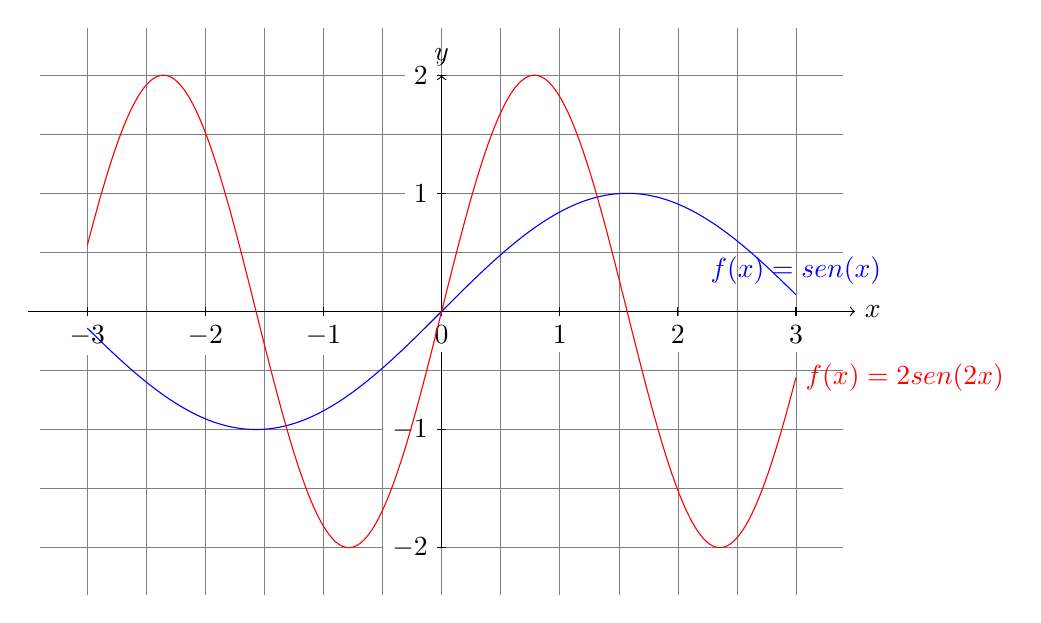
\begin{tikzpicture}[scale = 1.5]

        % Styles
        \tikzstyle{axes}=[]
        \tikzstyle{important line}=[very thick]
        \tikzstyle{information text}=[rounded corners,fill=red!10,inner sep=1ex]
        %The graphic
        %axes
        \draw[style=help lines,step=0.5cm] (-3.4,-2.4) grid (3.4,2.4);
        \begin{scope}[style=axes]
            \draw[->] (-3.5,0) -- (3.5,0) node[right] {$x$} coordinate(x axis);
            \draw[->] (0,-2) -- (0,2) node[above] {$y$} coordinate(y axis);
             \foreach \x/\xtext in {-3,-2,-1,0,1,2,3}
                \draw[xshift=\x cm] (0pt,1pt) -- (0pt,-1pt) node[below,fill=white] {$\xtext$};
            \foreach \y/\ytext in {-2,-1,1,2}
                \draw[yshift=\y cm] (1pt,0pt) -- (-1pt,0pt) node[left,fill=white] {$\ytext$};
        \end{scope}
        \draw [color=blue, domain=-3:3,samples = 300] plot(\x, { sin(\x r) } ) node[above]{$f(x)= sen(x) $};
        \draw [color=red, domain=-3:3,samples = 300] plot(\x, { 2*sin(2*\x r) } ) node[right]{$f(x)= 2sen(2x) $};
        % sin, cos , tan , cot , sec , cosec, asin , acos , atan
\end{tikzpicture}
\end{center}


\subsubsection{Coseno} \label{Cos}
En un triangulo rectángulo se define como la relación entre el cateto adyacente al
ángulo y la hipotenusa: $ cos(\alpha)= \frac{C.A}{H} $.

Como función, se expresa como $ cos(x) \text{ con  }x\in\mathbb{R} $.

Su dominio es: $ \mathbb{R} $ y su rango es: [-1,1].

Puede ser expresado como: $ A\times cos(n\times x) $, donde $A,n$son números reales
cualesquiera.

Su gráfica puede ser expandida o comprimida en el eje x mediante el valor de $n$,
con $ n \not = 0; si n>1 comprime $  y  expandida o comprimida en el eje y
mediante el valor de $ A $, con $ A \not = 0; si A>1 expande $




\begin{center}
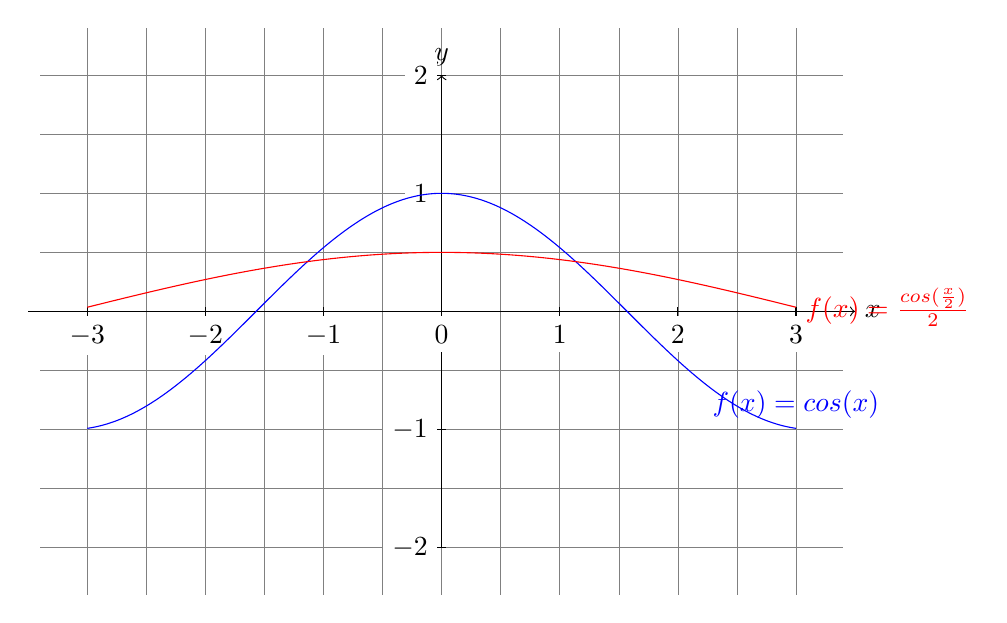
\begin{tikzpicture}[scale = 1.5]

        % Styles
        \tikzstyle{axes}=[]
        \tikzstyle{important line}=[very thick]
        \tikzstyle{information text}=[rounded corners,fill=red!10,inner sep=1ex]
        %The graphic
        %axes
        \draw[style=help lines,step=0.5cm] (-3.4,-2.4) grid (3.4,2.4);
        \begin{scope}[style=axes]
            \draw[->] (-3.5,0) -- (3.5,0) node[right] {$x$} coordinate(x axis);
            \draw[->] (0,-2) -- (0,2) node[above] {$y$} coordinate(y axis);
             \foreach \x/\xtext in {-3,-2,-1,0,1,2,3}
                \draw[xshift=\x cm] (0pt,1pt) -- (0pt,-1pt) node[below,fill=white] {$\xtext$};
            \foreach \y/\ytext in {-2,-1,1,2}
                \draw[yshift=\y cm] (1pt,0pt) -- (-1pt,0pt) node[left,fill=white] {$\ytext$};
        \end{scope}
        \draw [color=blue, domain=-3:3,samples = 300] plot(\x, { cos(\x r) } ) node[above]{$f(x)= cos(x) $};
        \draw [color=red, domain=-3:3,samples = 300] plot(\x, { 0.5*cos(0.5*\x r) } ) node[right]{$f(x)= \frac{ cos(\frac{x}{2} ) }{2} $};
        % sin, cos , tan , cot , sec , cosec, asin , acos , atan
\end{tikzpicture}
\end{center}




\subsubsection{Tangente} \label{Tan}
En un triangulo rectángulo se define como la relación entre el cateto opuesto y
el cateto adyacente del ángulo: $ tan(\alpha)= \frac{C.O}{C.A} $.

Como función, se expresa como $ tan(x) \text{ con  }x\in\mathbb{R}-{\frac{\pi}{2}+n\pi,n\in \mathbb{Z} } $.

Su dominio es: $ \mathbb{R} -{\frac{\pi}{2}+n\pi,n\in \mathbb{Z} } $ y su rango es: $ \mathbb{R} $.

Puede ser expresado como: $ A\times tan(n\times x) $, donde $A,n$son números reales
cualesquiera.

Su gráfica puede ser expandida o comprimida en el eje x mediante el valor de $n$,
con $ n \not = 0; si n>1 comprime $  y  expandida o comprimida en el eje y
mediante el valor de $ A $, con $ A \not = 0; si A>1 expande $

\begin{center}
    \begin{tikzpicture}[domain=-4:7]
        % x and y axes
        \draw[thick, ->] (-6,0)     -- (6,0)   node[right] {$x$};
        \draw[thick, ->] (0,-4.2)   -- (0,4.2) node[above] {$y$};
        % vertical asymptotes
        \draw[dashed, thick,red] (pi/2,-4.2)    --  (pi/2,4.2);
        \draw[dashed, thick,red] (3*pi/2,-4.2)  --  (3*pi/2,4.2);
        \draw[dashed, thick,red] (-pi/2,-4.2)   --  (-pi/2, 4.2);
        \draw[dashed, thick,red] (-3*pi/2,-4.2) --  (-3*pi/2, 4.2);
        % tangent between vertical asymptotes
        \draw[ thick,color=red, <->] plot [domain=-0.425*pi:0.425*pi] (\x,{tan(\x r)});
        \draw[ thick,color=red, <->] plot [domain= 0.573*pi:1.425*pi] (\x,{tan(\x r)});
        \draw[ thick,color=red, <->] plot [domain= -1.425*pi:-0.573*pi] (\x,{tan(\x r)});
        % x tick labels
        \node[below right] at (-3*pi/2, 0)  {$-\frac{3\pi}{2}$};
        \node[below right] at (-pi, 0)      {$-\pi$};
        \node[below right] at (-pi/2, 0)    {$-\frac{\pi}{2}$};
        \node[below right] at (0, 0)        {$0$};
        \node[below right] at (pi/2, 0)     {$\frac{\pi}{2}$};
        \node[below right] at (pi, 0)       {$\pi$};
        \node[below right] at (3*pi/2, 0)   {$\frac{3\pi}{2}$};
    \end{tikzpicture}
\end{center}


\subsubsection{Cotangente} \label{Cot}

En un triangulo rectángulo se define como la relación entre el cateto adyacente y
el cateto opuesto del  ángulo: $\displaystyle cot(\alpha)= \frac{1}{tan(\alpha)} \frac{C.A}{C.O} $.

Como función, se expresa como $ cot(x) \text{ con  }x\in\mathbb{R}-{n\pi,n\in \mathbb{Z} } $.

Su dominio es: $ \mathbb{R} -{n\pi,n\in \mathbb{Z} } $ y su rango es: $ \mathbb{R} $.

Puede ser expresado como: $ A\times cot(n\times x) $, donde $A,n$son números reales
cualesquiera.

Su gráfica puede ser expandida o comprimida en el eje x mediante el valor de $n$,
con $ n \not = 0; si n>1 comprime $  y  expandida o comprimida en el eje y
mediante el valor de $ A $, con $ A \not = 0; si A>1 expande $


\begin{center}
    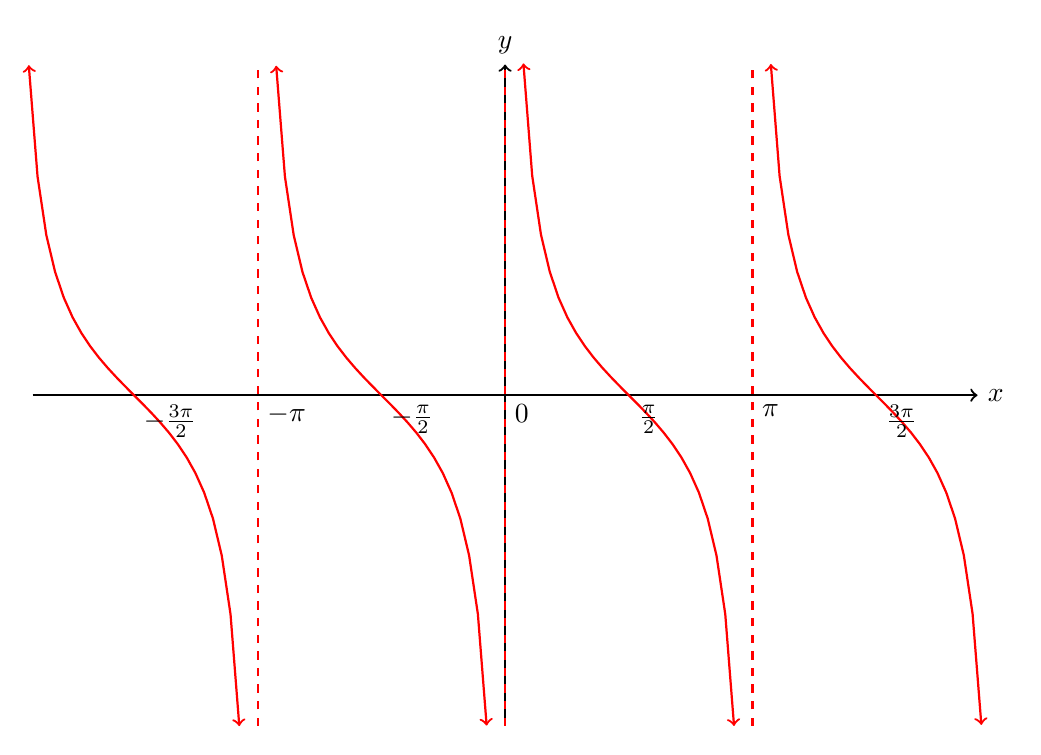
\begin{tikzpicture}[domain=-4:7]         % x and y axes
        \draw[thick, ->] (-6,0)     -- (6,0)   node[right] {$x$};
        \draw[thick, ->] (0,-4.2)   -- (0,4.2) node[above] {$y$};
        % vertical asymptotes
        \draw[dashed, thick,red] (pi,-4.2)    --  (pi,4.2);
        \draw[dashed, thick,red] (0,-4.2)  --  (0,4.2);
        \draw[dashed, thick,red] (-pi,-4.2)   --  (-pi, 4.2);

        % tangent between vertical asymptotes
        \draw[ thick,color=red, <->] plot [domain= -6.049:-3.375] (\x,{cot(\x r)});
        \draw[ thick,color=red, <->] plot [domain=-2.907:-0.234] (\x,{cot(\x r)});
        \draw[ thick,color=red, <->] plot [domain=0.233:2.908] (\x,{cot(\x r)});
        \draw[ thick,color=red, <->] plot [domain= 3.375:6.049] (\x,{cot(\x r)});
        % x tick labels
        \node[below right] at (-3*pi/2, 0)  {$-\frac{3\pi}{2}$};
        \node[below right] at (-pi, 0)      {$-\pi$};
        \node[below right] at (-pi/2, 0)    {$-\frac{\pi}{2}$};
        \node[below right] at (0, 0)        {$0$};
        \node[below right] at (pi/2, 0)     {$\frac{\pi}{2}$};
        \node[below right] at (pi, 0)       {$\pi$};
        \node[below right] at (3*pi/2, 0)   {$\frac{3\pi}{2}$};
    \end{tikzpicture}
\end{center}



\subsubsection{Cosecante} \label{csc}
En un triangulo rectángulo se define como la relación entre la hipotenusa y el
cateto opuesto al ángulo:  $ \displaystyle csc(\alpha)=\frac{1}{sen(\alpha)}  \frac{H}{C.O} $.

Como función, se expresa como $ csc(x) \text{ con  }x\in\mathbb{R} -{n\pi,n\in \mathbb{Z} }$.

Su dominio es: $ \mathbb{R}-{n\pi,n\in \mathbb{Z} }$ y su rango es: $\mathbb{R}-(-1,1)$.

Puede ser expresado como: $ A\times csc(n\times x) $, donde $A,n$son números reales
cualesquiera.

Su gráfica puede ser expandida o comprimida en el eje x mediante el valor de $n$,
con $ n \not = 0; si n>1 comprime $  y  expandida o comprimida en el eje y
mediante el valor de $ A $, con $ A \not = 0; si A>1 expande $


\begin{center}
    \begin{tikzpicture}[domain=-4:7]
        % x and y axes
        \draw[thick, ->] (-6,0)     -- (6,0)   node[right] {$x$};
        \draw[thick, ->] (0,-4.2)   -- (0,4.2) node[above] {$y$};
        % vertical asymptotes
        \draw[dashed, thick,red] (pi,-4.2)    --  (pi,4.2);
        \draw[dashed, thick,red] (0,-4.2)  --  (0,4.2);
        \draw[dashed, thick,red] (-pi,-4.2)   --  (-pi, 4.2);

        % tangent between vertical asymptotes
        \draw[ thick,color=red, <->] plot [domain= -6.049:-3.375] (\x,{1/sin(\x r)});
        \draw[ thick,color=red, <->] plot [domain=-2.907:-0.234] (\x,{1/sin(\x r)});
        \draw[ thick,color=red, <->] plot [domain=0.233:2.908] (\x,{1/sin(\x r)});
        \draw[ thick,color=red, <->] plot [domain= 3.375:6.049] (\x,{1/sin(\x r)});
        % x tick labels
        \node[below right] at (-3*pi/2, 0)  {$-\frac{3\pi}{2}$};
        \node[below right] at (-pi, 0)      {$-\pi$};
        \node[below right] at (-pi/2, 0)    {$-\frac{\pi}{2}$};
        \node[below right] at (0, 0)        {$0$};
        \node[below right] at (pi/2, 0)     {$\frac{\pi}{2}$};
        \node[below right] at (pi, 0)       {$\pi$};
        \node[below right] at (3*pi/2, 0)   {$\frac{3\pi}{2}$};
    \end{tikzpicture}
\end{center}


\subsubsection{Secante} \label{Sec}
En un triangulo rectángulo se define como la relación entre la hipotenusa y el
cateto adyacente al ángulo:  $\displaystyle sec(\alpha)=\frac{1}{cos(\alpha)}  \frac{H}{C.A} $.

Como función, se expresa como $ sec(x) \text{ con  }x\in\mathbb{R} -{\frac{\pi}{2}+n\pi,n\in \mathbb{Z} }$.

Su dominio es: $ \mathbb{R} -{\frac{\pi}{2}+n\pi,n\in \mathbb{Z} }$ y su rango es: $\mathbb{R}-(-1,1)$.

Puede ser expresado como: $ A\times sec(n\times x) $, donde $A,n$son números reales
cualesquiera.

Su gráfica puede ser expandida o comprimida en el eje x mediante el valor de $n$,
con $ n \not = 0; si n>1 comprime $  y  expandida o comprimida en el eje y
mediante el valor de $ A $, con $ A \not = 0; si A>1 expande $

\begin{center}
    \begin{tikzpicture}[domain=-4:7]
        % x and y axes
        \draw[thick, ->] (-6,0)     -- (6,0)   node[right] {$x$};
        \draw[thick, ->] (0,-4.2)   -- (0,4.2) node[above] {$y$};
        % vertical asymptotes
        \draw[dashed, thick,red] (pi/2,-4.2)    --  (pi/2,4.2);
        \draw[dashed, thick,red] (3*pi/2,-4.2)  --  (3*pi/2,4.2);
        \draw[dashed, thick,red] (-pi/2,-4.2)   --  (-pi/2, 4.2);
        \draw[dashed, thick,red] (-3*pi/2,-4.2) --  (-3*pi/2, 4.2);
        % tangent between vertical asymptotes
        \draw[ thick,color=red, <->] plot [domain=-0.425*pi:0.425*pi] (\x,{1/cos(\x r)});
        \draw[ thick,color=red, <->] plot [domain= 0.573*pi:1.425*pi] (\x,{1/cos(\x r)});
        \draw[ thick,color=red, <->] plot [domain= -1.425*pi:-0.573*pi] (\x,{1/cos(\x r)});
        % x tick labels
        \node[below right] at (-3*pi/2, 0)  {$-\frac{3\pi}{2}$};
        \node[below right] at (-pi, 0)      {$-\pi$};
        \node[below right] at (-pi/2, 0)    {$-\frac{\pi}{2}$};
        \node[below right] at (0, 0)        {$0$};
        \node[below right] at (pi/2, 0)     {$\frac{\pi}{2}$};
        \node[below right] at (pi, 0)       {$\pi$};
        \node[below right] at (3*pi/2, 0)   {$\frac{3\pi}{2}$};
    \end{tikzpicture}
\end{center}

